
\documentclass[aps,amsmath,onecolumn,amssymb]{revtex4}
%\documentclass{iopart}
\usepackage{amssymb}
\usepackage{amsthm}
\usepackage{amsfonts}
\usepackage{complexity}
\usepackage{graphicx}% Include figure files
\usepackage{dcolumn}% Align table columns on decimal point
\usepackage{bm}% bold math
\usepackage{hyperref}
% \usepackage{color}
%\usepackage{iopams}
\usepackage{enumerate}
\usepackage{algorithm}
\usepackage{algpseudocode}
    \renewcommand{\algorithmicrequire}{\textbf{Input:}}
    \renewcommand{\algorithmicensure}{\textbf{Output:}}
    \newcommand{\inlinecomment}[1]{\Comment {\footnotesize #1} \normalsize}
    \newcommand{\linecomment}[1]{\State \(\triangleright\) {\footnotesize #1} \normalsize}
    %\renewcommand{\algorithmiccomment}[1]{\State\(\triangleright\) #1}
    
\usepackage{multirow}



\newtheorem{theorem}{Theorem}
\newtheorem{lemma}{Lemma}
\newtheorem{definition}{Definition}
\newtheorem{corollary}{Corollary}
%    Q-circuit version 2
%    Copyright (C) 2004  Steve Flammia & Bryan Eastin
%    Last modified on: 9/16/2011
%
%    This program is free software; you can redistribute it and/or modify
%    it under the terms of the GNU General Public License as published by
%    the Free Software Foundation; either version 2 of the License, or
%    (at your option) any later version.
%
%    This program is distributed in the hope that it will be useful,
%    but WITHOUT ANY WARRANTY; without even the implied warranty of
%    MERCHANTABILITY or FITNESS FOR A PARTICULAR PURPOSE.  See the
%    GNU General Public License for more details.
%
%    You should have received a copy of the GNU General Public License
%    along with this program; if not, write to the Free Software
%    Foundation, Inc., 59 Temple Place, Suite 330, Boston, MA  02111-1307  USA

% Thanks to the Xy-pic guys, Kristoffer H Rose, Ross Moore, and Daniel Müllner,
% for their help in making Qcircuit work with Xy-pic version 3.8.  
% Thanks also to Dave Clader, Andrew Childs, Rafael Possignolo, Tyson Williams,
% Sergio Boixo, Cris Moore, Jonas Anderson, and Stephan Mertens for helping us test 
% and/or develop the new version.

\usepackage[color]{xy}
\UseCrayolaColors
\xyoption{matrix}
\xyoption{frame}
\xyoption{arrow}
\xyoption{arc}

\usepackage{ifpdf}
\ifpdf
\else
\PackageWarningNoLine{Qcircuit}{Qcircuit is loading in Postscript mode.  The Xy-pic options ps and dvips will be loaded.  If you wish to use other Postscript drivers for Xy-pic, you must modify the code in Qcircuit.tex}
%    The following options load the drivers most commonly required to
%    get proper Postscript output from Xy-pic.  Should these fail to work,
%    try replacing the following two lines with some of the other options
%    given in the Xy-pic reference manual.
\xyoption{ps}
\xyoption{dvips}
\fi

% The following resets Xy-pic matrix alignment to the pre-3.8 default, as
% required by Qcircuit.
\entrymodifiers={!C\entrybox}

%\newcommand{\bra}[1]{{\left\langle{#1}\right\vert}}
%\newcommand{\ket}[1]{{\left\vert{#1}\right\rangle}}
    % Defines Dirac notation. %7/5/07 added extra braces so that the commands will work in subscripts.
\newcommand{\qw}[1][-1]{\ar @{-} [0,#1]}
\newcommand{\eqw}[1][-1]{\ar @{-} @[Red] [0,#1]}
    % Defines a wire that connects horizontally.  By default it connects to the object on the left of the current object.
    % WARNING: Wire commands must appear after the gate in any given entry.
\newcommand{\qwx}[1][-1]{\ar @{-} [#1,0]}
    % Defines a wire that connects vertically.  By default it connects to the object above the current object.
    % WARNING: Wire commands must appear after the gate in any given entry.
\newcommand{\cw}[1][-1]{\ar @{=} [0,#1]}
    % Defines a classical wire that connects horizontally.  By default it connects to the object on the left of the current object.
    % WARNING: Wire commands must appear after the gate in any given entry.
\newcommand{\cwx}[1][-1]{\ar @{=} [#1,0]}
    % Defines a classical wire that connects vertically.  By default it connects to the object above the current object.
    % WARNING: Wire commands must appear after the gate in any given entry.
\newcommand{\gate}[1]{*+<.6em>{#1} \POS ="i","i"+UR;"i"+UL **\dir{-};"i"+DL **\dir{-};"i"+DR **\dir{-};"i"+UR **\dir{-},"i" \qw}
\newcommand{\eboxgate} [1]{*+<.6em>{#1} \POS ="i","i"+UR;"i"+UL **[red]\dir{-};"i"+DL **[red]\dir{-};"i"+DR **[red]\dir{-};"i"+UR **[red]\dir{-},"i" \eqw}
\newcommand{\circgate}[1]{*+<0.6em>[o][F-]{#1} \eqw}
\newcommand{\ecircgate}[1]{*+<0.6em>[o][F-:red]{#1} \eqw}
\newcommand{\filtergt}[1]{\eboxgate{\scriptscriptstyle{#1}}}
\newcommand{\idealdec}{*+<1.2em>{\phantom{*}} \POS ="i","i"+UL;"i"+DL **[red]\dir{-};"i"+R **[red]\dir{-};"i"+UL **[red]\dir{-},"i" \eqw}

    % Boxes the argument, making a gate.
\newcommand{\meter}{*=<1.8em,1.4em>{\xy ="j","j"-<.778em,.322em>;{"j"+<.778em,-.322em> \ellipse ur,_{}},"j"-<0em,.4em>;p+<.5em,.9em> **\dir{-},"j"+<2.2em,2.2em>*{},"j"-<2.2em,2.2em>*{} \endxy} \POS ="i","i"+UR;"i"+UL **\dir{-};"i"+DL **\dir{-};"i"+DR **\dir{-};"i"+UR **\dir{-},"i" \qw}
    % Inserts a measurement meter.
    % In case you're wondering, the constants .778em and .322em specify
    % one quarter of a circle with radius 1.1em.
    % The points added at + and - <2.2em,2.2em> are there to strech the
    % canvas, ensuring that the size is unaffected by erratic spacing issues
    % with the arc.
\newcommand{\measure}[1]{*+[F-:<.9em>]{#1} \qw}
    % Inserts a measurement bubble with user defined text.
\newcommand{\measuretab}[1]{*{\xy*+<.6em>{#1}="e";"e"+UL;"e"+UR **\dir{-};"e"+DR **\dir{-};"e"+DL **\dir{-};"e"+LC-<.5em,0em> **\dir{-};"e"+UL **\dir{-} \endxy} \qw}
    % Inserts a measurement tab with user defined text.
\newcommand{\measureD}[1]{*{\xy*+=<0em,.1em>{#1}="e";"e"+UR+<0em,.25em>;"e"+UL+<-.5em,.25em> **\dir{-};"e"+DL+<-.5em,-.25em> **\dir{-};"e"+DR+<0em,-.25em> **\dir{-};{"e"+UR+<0em,.25em>\ellipse^{}};"e"+C:,+(0,1)*{} \endxy} \qw}
\newcommand{\emeasureD}[1]{*{\xy*+=<0em,.1em>{#1}="e";"e"+UR+<0em,.25em>;"e"+UL+<-.5em,.25em> **[red]\dir{-};"e"+DL+<-.5em,-.25em> **[red]\dir{-};"e"+DR+<0em,-.25em> **[red]\dir{-};{"e"+UR+<0em,.25em>\ellipse{}};"e"+C:,+(0,1)*{} \endxy} \qw}
    % Inserts a D-shaped measurement gate with user defined text.
\newcommand{\multimeasure}[2]{*+<1em,.9em>{\hphantom{#2}} \qw \POS[0,0].[#1,0];p !C *{#2},p \drop\frm<.9em>{-}}
    % Draws a multiple qubit measurement bubble starting at the current position and spanning #1 additional gates below.
    % #2 gives the label for the gate.
    % You must use an argument of the same width as #2 in \ghost for the wires to connect properly on the lower lines.
\newcommand{\multimeasureD}[2]{*+<1em,.9em>{\hphantom{#2}} \POS [0,0]="i",[0,0].[#1,0]="e",!C *{#2},"e"+UR-<.8em,0em>;"e"+UL **\dir{-};"e"+DL **\dir{-};"e"+DR+<-.8em,0em> **\dir{-};{"e"+DR+<0em,.8em>\ellipse^{}};"e"+UR+<0em,-.8em> **\dir{-};{"e"+UR-<.8em,0em>\ellipse^{}},"i" \qw}
    % Draws a multiple qubit D-shaped measurement gate starting at the current position and spanning #1 additional gates below.
    % #2 gives the label for the gate.
    % You must use an argument of the same width as #2 in \ghost for the wires to connect properly on the lower lines.
\newcommand{\control}{*!<0em,.025em>-=-<.2em>{\bullet}}
    % Inserts an unconnected control.
\newcommand{\controlo}{*+<.01em>{\xy -<.095em>*\xycircle<.19em>{} \endxy}}
    % Inserts a unconnected control-on-0.
\newcommand{\ctrl}[1]{\control \qwx[#1] \qw}
    % Inserts a control and connects it to the object #1 wires below.
\newcommand{\ctrlo}[1]{\controlo \qwx[#1] \qw}
    % Inserts a control-on-0 and connects it to the object #1 wires below.
\newcommand{\targ}{*+<.02em,.02em>{\xy ="i","i"-<.39em,0em>;"i"+<.39em,0em> **\dir{-}, "i"-<0em,.39em>;"i"+<0em,.39em> **\dir{-},"i"*\xycircle<.4em>{} \endxy} \qw}
    % Inserts a CNOT target.
\newcommand{\qswap}{*=<0em>{\times} \qw}
    % Inserts half a swap gate.
    % Must be connected to the other swap with \qwx.
\newcommand{\multigate}[2]{*+<1em,.9em>{\hphantom{#2}} \POS [0,0]="i",[0,0].[#1,0]="e",!C *{#2},"e"+UR;"e"+UL **\dir{-};"e"+DL **\dir{-};"e"+DR **\dir{-};"e"+UR **\dir{-},"i" \qw}
    % Draws a multiple qubit gate starting at the current position and spanning #1 additional gates below.
    % #2 gives the label for the gate.
    % You must use an argument of the same width as #2 in \ghost for the wires to connect properly on the lower lines.
\newcommand{\ghost}[1]{*+<1em,.9em>{\hphantom{#1}} \qw}
    % Leaves space for \multigate on wires other than the one on which \multigate appears.  Without this command wires will cross your gate.
    % #1 should match the second argument in the corresponding \multigate.
\newcommand{\push}[1]{*{#1}}
    % Inserts #1, overriding the default that causes entries to have zero size.  This command takes the place of a gate.
    % Like a gate, it must precede any wire commands.
    % \push is useful for forcing columns apart.
    % NOTE: It might be useful to know that a gate is about 1.3 times the height of its contents.  I.e. \gate{M} is 1.3em tall.
    % WARNING: \push must appear before any wire commands and may not appear in an entry with a gate or label.
\newcommand{\gategroup}[6]{\POS"#1,#2"."#3,#2"."#1,#4"."#3,#4"!C*+<#5>\frm{#6}}
    % Constructs a box or bracket enclosing the square block spanning rows #1-#3 and columns=#2-#4.
    % The block is given a margin #5/2, so #5 should be a valid length.
    % #6 can take the following arguments -- or . or _\} or ^\} or \{ or \} or _) or ^) or ( or ) where the first two options yield dashed and
    % dotted boxes respectively, and the last eight options yield bottom, top, left, and right braces of the curly or normal variety.  See the Xy-pic reference manual for more options.
    % \gategroup can appear at the end of any gate entry, but it's good form to pick either the last entry or one of the corner gates.
    % BUG: \gategroup uses the four corner gates to determine the size of the bounding box.  Other gates may stick out of that box.  See \prop.

\newcommand{\rstick}[1]{*!L!<-.5em,0em>=<0em>{#1}}
    % Centers the left side of #1 in the cell.  Intended for lining up wire labels.  Note that non-gates have default size zero.
\newcommand{\lstick}[1]{*!R!<.5em,0em>=<0em>{#1}}
    % Centers the right side of #1 in the cell.  Intended for lining up wire labels.  Note that non-gates have default size zero.
\newcommand{\ustick}[1]{*!D!<0em,-.5em>=<0em>{#1}}
    % Centers the bottom of #1 in the cell.  Intended for lining up wire labels.  Note that non-gates have default size zero.
\newcommand{\dstick}[1]{*!U!<0em,.5em>=<0em>{#1}}
    % Centers the top of #1 in the cell.  Intended for lining up wire labels.  Note that non-gates have default size zero.
\newcommand{\Qcircuit}{\xymatrix @*=<0em>}
    % Defines \Qcircuit as an \xymatrix with entries of default size 0em.
\newcommand{\link}[2]{\ar @{-} [#1,#2]}
    % Draws a wire or connecting line to the element #1 rows down and #2 columns forward.
\newcommand{\pureghost}[1]{*+<1em,.9em>{\hphantom{#1}}}
    % Same as \ghost except it omits the wire leading to the left. 
%%%%%%%%%%%%%%%%%%%%%%%%%%%%%%%%%%%%%%%%%%%%%%%%%%%%%%%%%%%%%%%%%%%%%%%%%%%%%%%%%%%%%%%%%%
\newcommand{\multiprepareC}[2]{*+<1em,.9em>{\hphantom{#2}}\save[0,0].[#1,0];p\save !C
  *{#2},p+RU+<0em,0em>;+LU+<+.8em,0em> **\dir{-}\restore\save +RD;+RU **\dir{-}\restore\save
  +RD;+LD+<.8em,0em> **\dir{-} \restore\save +LD+<0em,.8em>;+LU-<0em,.8em> **\dir{-} \restore \POS
  !UL*!UL{\cir<.9em>{u_r}};!DL*!DL{\cir<.9em>{l_u}}\restore}
   % Draws a multiple qubit reverse-D-shaped preparation gate starting at the current position and spanning #1 additional gates below.
   % #2 gives the label for the gate.
   % You must use an argument of the same width as #2 in \pureghost for the wires to connect properly on
% the lower lines.
\newcommand{\prepareC}[1]{*{\xy*+=+<.5em>{\vphantom{#1\rule{0em}{.1em}}}*\cir{l^r};p\save*!L{#1} \restore\save+UC;+UC+<.5em,0em>*!L{\hphantom{#1}}+R **\dir{-} \restore\save+DC;+DC+<.5em,0em>*!L{\hphantom{#1}}+R **\dir{-} \restore\POS+UC+<.5em,0em>*!L{\hphantom{#1}}+R;+DC+<.5em,0em>*!L{\hphantom{#1}}+R **\dir{-} \endxy}}
   % Inserts a reverse-D-shaped preparation gate with user defined text.
\newcommand{\poloFantasmaCn}[1]{{{}^{#1}_{\phantom{#1}}}}


%%%%%%%%%%%%%%%%%%%%%%% a bit nicer hypelinks %%%%%%%%%%%%%%%%%%%%%%%%%%%%%

\usepackage[usenames,dvipsnames]{xcolor}
\hypersetup{
    colorlinks=true,       % false: boxed links; true: colored links
    linkcolor=Maroon,          % color of internal links (change box color with linkbordercolor)
    citecolor=OliveGreen,        % color of links to bibliography
    filecolor=magenta,      % color of file links
    urlcolor=Blue           % color of external links
}

%%%%%%%%%%%%%%%%%%%%%%% a bit nicer hypelinks %%%%%%%%%%%%%%%%%%%%%%%%%%%%%

\begin{document}

\def\ket#1{\left|#1\right\rangle}
\def\bra#1{\langle#1|}
\newcommand{\ketbra}[2]{|#1\rangle\!\langle#2|}
\newcommand{\braket}[2]{\langle#1|#2\rangle}
% \newcommand{\note}[1]{({\bf note: #1})}
\newcommand{\prob}[1]{{\rm Pr}\left(#1 \right)}
% \newcommand{\Tr}[1]{{\rm Tr}\!\left[#1 \right]}
\newcommand{\expect}[2]{{\mathbb{E}_{#2}}\!\left\{#1 \right\}}
\newcommand{\var}[2]{{\mathbb{V}_{#2}}\!\left\{#1 \right\}}

\newcommand{\sinc}{\operatorname{sinc}}

% fix: supported only for revtex
%\newcommand{\openone}{\mathbb{I}}
% fix: unsupported with iopart
%\newcommand{\eqref}[1]{(\ref{#1})}

\newcommand{\sde}{\mathrm{sde}}
\newcommand{\Z}{\mathbb{Z}}
\newcommand{\RR}{\mathbb{R}}
\newcommand{\w}{\omega}
\newcommand{\Kap}{\kappa}

\newcommand{\Tchar}{$T$}
\newcommand{\T}{\Tchar~}
\newcommand{\TT}{\mathrm{T}}
\newcommand{\ClT}{\{{\rm Clifford}, \Tchar\}~}
\newcommand{\Tcount}{\Tchar--count~}
\newcommand{\Tcountper}{\Tchar--count}
\newcommand{\Tcounts}{\Tchar--counts~}
\newcommand{\Tdepth}{\Tchar--depth~}
\newcommand{\Zr}{\Z[i,1/\sqrt{2}]}
\newcommand{\ve}{\varepsilon}

\newcommand{\eq}[1]{\hyperref[eq:#1]{(\ref*{eq:#1})}}
\renewcommand{\sec}[1]{\hyperref[sec:#1]{Section~\ref*{sec:#1}}}
\newcommand{\app}[1]{\hyperref[app:#1]{Appendix~\ref*{app:#1}}}
\newcommand{\fig}[1]{\hyperref[fig:#1]{Figure~\ref*{fig:#1}}}
\newcommand{\thm}[1]{\hyperref[thm:#1]{Theorem~\ref*{thm:#1}}}
\newcommand{\lem}[1]{\hyperref[lem:#1]{Lemma~\ref*{lem:#1}}}
\newcommand{\tab}[1]{\hyperref[tab:#1]{Table~\ref*{tab:#1}}}
\newcommand{\cor}[1]{\hyperref[cor:#1]{Corollary~\ref*{cor:#1}}}
\newcommand{\alg}[1]{\hyperref[alg:#1]{Algorithm~\ref*{alg:#1}}}
\newcommand{\defn}[1]{\hyperref[def:#1]{Definition~\ref*{def:#1}}}


\newcommand{\targfix}{\qw {\xy {<0em,0em> \ar @{ - } +<.39em,0em>
\ar @{ - } -<.39em,0em> \ar @{ - } +
<0em,.39em> \ar @{ - }
-<0em,.39em>},<0em,0em>*{\rule{.01em}{.01em}}*+<.8em>\frm{o}
\endxy}}

\newenvironment{proofof}[1]{\begin{trivlist}\item[]{\flushleft\it
Proof of~#1.}}
{\qed\end{trivlist}}


\newcommand{\cu}[1]{{\textcolor{red}{#1}}}
\newcommand{\tout}[1]{{}}
% \newcommand{\beq}{\begin{equation}}
% \newcommand{\eeq}{\end{equation}}
% \newcommand{\beqa}{\begin{eqnarray}}
\newcommand{\good}{{\rm good}}
\newcommand{\bad}{{\rm bad}}
% \newcommand{\eeqa}{\end{eqnarray}}

\newcommand{\id}{\openone}
%\newcommand{\id}{\mathbb{I}}
\title{Efficient Online Quantum Bayesian Inference}
\author{Nathan Wiebe$^\dagger$}
\author{Christopher Granade$^{*+}$}
\affiliation{$^\dagger$Quantum Architectures and Computation Group, Microsoft Research, Redmond, WA (USA)}
\affiliation{$^*$Institute for quantum computing, Waterloo, ON (Canada)}
\affiliation{$^+$Center for engineered quantum systems, Sydney, NSW (Australia)}
\begin{abstract}
We present a new quantum algorithm for online quantum approximate Bayesian inference that can efficiently estimate the low order moments of the posterior distribution in an online setting modulo reasonable assumptions on the likelihood function.  Our method does so by sampling from the distribution over these single hypotheses to learn a simple model for the posterior distribution, which allows our algorithm to learn in an online fashion without measurement errors causing the posterior distribution to be lost.  We further show that the success probability of our algorithm is essentially optimal by showing that an asymptotic improvement to the algorithm's success probability would violate lower bounds for unstructured search and also provide quantum methods for adaptive experiment design and learning in the presence of stochastically varying latent variables.\end{abstract}
\maketitle
\section{Introduction}
Data processing has emerged within the last few years to be a problem of central importance within both academic circles and industry.  The need for ever more sophisticated methods for processing data arose from the fact that modern experiments produce huge amounts of data and properly inferring information from huge data sets can require substantial computational power.  A natural question to ask is whether quantum technologies can help quell the insatiable demand on computational time that statistical inference creates.  We present here evidence that quantum computing can be used to speed up statistical inference relative to classical methods and show that limits exist on the extent to which such methods can be accelerated.  

In particular, we focus on accelerating Bayesian inference.  Bayes' rule is the heart of Bayesian inference, which gives the correct way to update a prior distribution that describes the experimentalist's initial beliefs about a system model when a piece of experimental evidence is received.  If $E$ be a piece of evidence (an observable variable) and $x$ denotes a candidate model for the experimental system (a latent or hidden variable) then Bayes' rule states that the probability that the model is valid given the evidence (denoted $P(x|E)$) is 
\begin{equation}
P(x|E)= \frac{P(E|x) P(x)}{\int_x P(E|x) P(x)\mathrm{d}x}= \frac{P(E|x) P(x)}{\langle P(E|x), P(x) \rangle},\label{eq:Bayes}
\end{equation}
where $P(E|x)$ is known as the likelihood function and is assumed to either be either numerically or inferred emperically.
This form of learning has a number of advantages for applications in quantum information processing.  Firstly, it is highly robust to noise and experimental imperfections.  Secondly, it is broadly applicable to almost every data processing problem.  Finally, Bayesian inference provides a probability distribution rather than a point estimate of the model. This allows the uncertainty in the inferred parameter to be directly computed.



There are several features that can make Bayesian inference computationally expensive, especially for scientific applications.  Perhaps the biggest contributor to the cost of these algorithms is the dimensionality of the model space.  Typically the model $x$ is parameterized by a vector in $\mathbb{R}^d$, which means that precisely performing an update requires integrating over an infinite number of hypotheses.  Such integrals are often intractable, which limits the applicability of exact Bayesian inference.  %Another important issue is that the likelihood function is also often intractable in absentia of quantum computing.  These features make exact Bayesian inference challenging.

A natural question to ask at this point is whether quantum computing could make inference tractable.  This issue is has been recently discussed in~\cite{LYC14}, which uses ideas from quantum rejection sampling~\cite{HHL09,ORR13} to accelerate the inference process.  Their work leaves a number of important issues open.  The method has success probability that shrinks exponentially with the number of updates attempted.  Furthermore, the algorithm cannot be applied in an online fashion nor can it be applied to continuous problems or those with stochastically varying latent variables.  We address these issues here by providing a quantum algorithm that can implement Bayesian inference in an online fashion by periodically classically caching a model of the posterior distribution.  This approach to learning not only generalizes the prior Bayesian inference work, but also generalizes Grover's search to scenarios where queries do not provide definitive evidence about the marked state.  We provide a complete description of this in the following.


%\begin{equation}
%P(x) \approx \sum_j w_j \delta_{x-x_j}.
%\end{equation}


%---------------------------------------------------------------------
\section{Quantum Bayesian updating}
%---------------------------------------------------------------------
Quantum theory is often viewed as a generalization of classical probability theory, which suggests that the notion of a Bayesian update may require re--assessment in quantum computing.  Indeed, there are several natural analogues of quantum Bayesian updating that can be thought of in a quantum setting.
Our objective in this section is to provide a definition for what we mean by a quantum Bayesian update and show a concrete protocol for implementing a quantum Bayesian update.  We will then show that this method cannot generically be efficient and furthermore that asymptotic improvements to the algorithm or an inexpensive error correction algorithm for its faults would violate lower bounds on Grover's search.  These results motivate our definition of ``semi--classical'' Bayesian updating in the subsequent section.

 A key assumption that we make here and in the subsequent text is that the visible and latent variables are discrete.  In other words, we assume that each experiment has a discrete set of outcomes and there are a discrete set of hypotheses that could explain the data.  We then use these assumptions to make the following definition of a quantum Bayesian update.
\begin{definition}\label{def:qbayes}
A quantum Bayesian update of a prior state $\sum_x \sqrt{P(x)} \ket{x}$ performs, for observable variable $E$ and likelihood function $P(E|x)$, the map 
$$\sum_x \sqrt{P(x)} \ket{x}\mapsto  \sum_x \sqrt{P(x|E)} \ket{x}. $$
\end{definition}

In order to formalize this notion of quantum Bayesian updating within an oracular setting we will further make a pair of assumptions.
%The idea behind this method is to implement Bayes' rule by using ideas from quantum rejection sampling, which is also used in algorithms like the Harrow, Hassidim and Lloyd algorithm for solving systems of linear equations~\cite{HHL09}.  In order to apply the algorithm we will assume the following
\begin{enumerate}
\item There exists a self-inverse quantum oracle, $O_E$, that computes the likelihood function as a bit string in a quantum register: $O_E\ket{x}\ket{y} = \ket{x}\ket{y\oplus P(E|x)}$.
\item A constant $\Gamma_E$ is known such that $P(E|x) \le \Gamma_E \le 1$ for all $x$.
\end{enumerate}
%The use of a value $\Gamma_E<1$ allows the  from pure rejection sampling to importance sampling where the instrumental distribution is the distribution $\openone/\Gamma_E$.  In this vein, $\Gamma_E$ couls also be taken to be a non--trivial function of $x$.  This can reduce the posterior variance in the estimate of the true model parameter but we will not consider this case in detail as it purposefully distorts the posterior distribution.


An interesting consequence of the above assumptions and~\defn{qbayes} is that in general the Bayesian update is non-unitary when working on this space.  This means that we cannot  implement a quantum Bayesian update deterministically without dilating the space.
The following lemma discusses how to implement such a non--deterministic quantum Bayesian update.  It can also be thought of as a generalization of the result of~\cite{LYC14} to an oracular setting.

\begin{lemma}
Given an initial state $\sum_x \sqrt{P(x)} \ket{x}$ and $\Gamma_E : P(E|x) \le \Gamma_E$ the state $\sum_x \sqrt{P(x|E)} \ket{x}$ can be prepared using an expected number of queries to $O_E$ that is in $O(\sqrt{\Gamma_E/\langle P(x), P(E|x)\rangle})$.\label{lem:rejection}
\end{lemma}
\begin{proof}
Using a single call to $O_E$ and adding a sufficient number of ancilla qubits, we can transform the state $\sum_x \sqrt{P(x)} \ket{x}$ into
\begin{equation}
\sum_x \sqrt{P(x)} \ket{x} \ket{P(E|x)}\ket{0}.
\end{equation}
Then by applying $R_y(2 \sin^{-1}(P(E|x)/\Gamma_E))$ to the ancilla qubit we can enact
\begin{equation}
\sum_x \sqrt{P(x)} \ket{x} \ket{P(E|x)}\ket{0}\mapsto \sum_x \sqrt{P(x)} \ket{x} \ket{P(E|x)}\left(\sqrt{\frac{P(E|x)}{\Gamma_E}}\ket{1} + \sqrt{1-\frac{P(E|x)}{\Gamma_E}}\ket{0} \right).\label{eq:rejection}
\end{equation}
Next the right most qubit register is measured and if a result of $1$ is obtained then the resultant state is
\begin{equation}
\frac{\sum_{x} \sqrt{P(x) P(E|x)}\ket{x}}{\sqrt{\sum_x P(x)P(E|x)}},
\end{equation}
which gives a probability distribution that corresponds to that expected by Bayes' rule.  The probability of this occurring is $\sum_x P(x) P(E|x) /\Gamma_E$.

Since the process is heralded, amplitude amplification can be used to boost the probability of success for the successful branch quadratically~\cite{BHM+02}.  Thus the average number of queries is in $O(\sqrt{\Gamma_E/\langle P(x), P(E|x)\rangle})$ as claimed.
\end{proof}
If the Bayesian algorithm is used solely to post--process information then one update will suffice to give the posterior distribution.  In online settings many updates will be needed to reach the final posterior distribution.  If $L$ updates are required then the probability of all such updates succeeding given a sequence of observed variables $E_1,\ldots,E_L$ is at most
\begin{equation}
P_{\rm succ} \le \sum_x P(x) \left(\max_E \frac{P(E|x)}{\Gamma_E}\right)^L\le \sqrt{\sum_x P^2(x)\sum_x \left(\max_E \frac{P(E|x)}{\Gamma_E}\right)^{2L}}\le\sqrt{\sum_x \left(\max_E \frac{P(E|x)}{\Gamma_E}\right)^{2L}}.
\end{equation}
This shows that the probability of success generically will shrink exponentially with $L$.

The exponential decay of the success probability with $L$ can be mitigated to some extent through amplitude amplification on the condition that all $L$ updates are successful  This reduces the expected number of updates needed to 
\begin{equation}
O\left(\left({\sum_x P(x) \left(\min_E \frac{P(E|x)}{\Gamma_E}\right)^L}\right)^{-1/2}\right),
\end{equation}
but this strategy is obviously insufficient to rid the method of its exponentially shrinking success probability.  Furthermore, we will see that there are fundamental limitations to our ability to avoid or correct such failures.
%
%Assuming that the norm of the covariance matrix for $x$ is a constant then this means that the posterior mean (which as an unbiased estimator of the true model) can be computed to within error $\delta$ using the following number of samples
%\begin{equation}
%O\left(\left({\sum_x P(x) \left(\min_E \frac{P(E|x)}{\Gamma_E}\right)^L}\right)^{-1/2}\delta^{-2}\right).
%\end{equation}

%A quantum update can therefore be performed, non-deterministically, using an elementary circuit.  However, the success probability may be exponentially 
%small.  Strategies for combating this exponential decay of likelihood of success or correcting preparation errors are needed.  Nonetheless, we will see that %there are limitations to our ability to correct such failures.

The reason why the errors in quantum rejection sampling cannot, in general, be efficiently corrected stems from the fact that quantum Bayesian inference algorithm described in~\lem{rejection} can be thought of as a generalization of Grover's algorithm~\cite{Gro96}.  Grover's problem (with one marked element) seeks to find $x = {\rm argmax}( f(x))$ where $O(x)$ is a blackbox Boolean function that is promised to have a unique $x_{\rm mark}$ such that $O(x_{\rm mark})=1$.  The generalization to multiple marked elements is similar.  The reduction between the two problems is formally proved below.

\begin{lemma}\label{lem:reduce}
Grover's problem with $N$ items and $m$ marked items reduces to Bayesian inference on a prior on $\mathbb{R}^N$.
\end{lemma}
\begin{proof}
Let $O$ be a Boolean function that takes the value $1$ iff $x\in X_m$ where $|X_m|=m$.  Identifying the set $X_m$ by querying this function is equivalent to Grover's problem.  Consider the following likelihood function on a two--outcome space where $1$ corresponds to finding a marked state and $0$ corresponds to finding an un--marked state:
\begin{equation}
P(1|x) = \begin{cases} 1 & {\rm if~}x\in X_m\\ 0& {\rm otherwise} \end{cases}.\label{eq:reduceLikelihood}
\end{equation}
We also have that $P(0|x)=1-P(1|x)$, but this fact is not needed for the proof.

It is then easy to see that $P(1|x)=O(x)$ and thus a likelihood evaluation is equivalent to a query to $O$.  This means that we can solve Grover's problem using the following algorithm.  \begin{enumerate}
\item Set the prior to be $P(x) = 1/N$.
\item Set $E=1$, which corresponds to pretending that an experiment was performed that found a marked entry.  
\item Compute $P(x|E) \propto P(E|x)P(x)$.  
\item Output all $x$ such that $P(x|E)=1/m$.
\end{enumerate}

The validity of this algorithm is easy to verify from~\eq{Bayes} and it is clear that the posterior distribution is a uniform distribution over $x\in X_m$.  Since $|X_m|=m$ and $P(x)$ is uniform, all elements in the support of the posterior distribution have probability $1/m$ and thus Grover's problem can be solved using Bayesian inference.  This algorithm will succeed classically using $N$ queries to $O$, rather than the $N-m$ queries required in the worst case scenario if a Bayesian framework is not adopted.


\end{proof}

This reduction of Grover's problem to Bayesian inference brings with it tight lower bounds on the query complexity of solving the problem~\cite{BGH+96}.  This means that we can exploit these bounds to show limitations on our ability to perform Bayesian inference on a quantum computer and also our ability to correct erroneous measurements that occur in the application of the method of~\lem{rejection}.  The following theorem states two such restrictions, which show that the method of~\lem{rejection} cannot be trivially improved nor can its failures be inexpensively corrected.

\begin{theorem}
The following are impossible.
\begin{enumerate}
\item An algorithm capable of performing a quantum Bayesian update of an arbitrary pure quantum state of the form $\sum_{x=1}^N \alpha_x \ket{x}$ using $O(1)$ queries to $O_E$ with success probability $\omega(\sqrt{\sum_x |\alpha_x|^2 P(E|x)/\Gamma_E})$.
\item An algorithm that requires $o(\sqrt{N}/\log(N))$ queries to $O_E$ to correct a failure of an algorithm that performs a quantum Bayesian update on $\sum_{x=1}^N \alpha_x \ket{x}$ using $O(1)$ queries with probability of success $\Omega(\sqrt{\sum_x |\alpha_x|^2 P(E|x)/\Gamma_E})$.
\end{enumerate}
\end{theorem}
\begin{proof}
Seeking a contradiction, assume that there exists a quantum algorithm that can perform a Bayesian update with probability $\omega(\sqrt{\sum_x |\alpha_x|^2 P(E|x)})$ for any likelihood function $P(E|x)$.  Next, let us choose the likelihood function to be that used in~\eq{reduceLikelihood} in the reduction proof of~\lem{reduce} and take $\alpha_x =1/\sqrt{N}~\forall~x$.  It is clear from~\lem{rejection} that $\Gamma_E =1$ must be chosen for this problem.  Then by assumption the state $\ket{x_m}$, where $x_m \in X_m$, can be found with probability $\omega(\sqrt{\sum_x |\alpha_x|^2 P(E|x)})= \omega(1/\sqrt{N})$.  Since each application of the algorithm requires $O(1)$ queries, $o(\sqrt{N})$ queries are needed on average to learn $x_m$, which violates lower bounds for the average query complexity for Grover's problem~\cite{BGH+96}.  Therefore such a quantum Bayesian inference algorithm is impossible.


Again seeking a contradiction, consider the following likelihood function with outcomes $\{1,0\}$
\begin{equation}
P(1|x) = \begin{cases}
2/3, & x=x_m \\
1/3, & x\ne x_m
\end{cases},~P({0}|x) = 1-P(E|x)\label{eq:bayesgrover}
\end{equation}
For each $x$, $P(1|x)$ can be computed using a single query to $O$ and vice versa, thus a query to this likelihood function is equivalent to a call to $O$.
Thus~\eq{Bayes} gives that the posterior probability after measuring $1$ is
\begin{equation}
\frac{2P(x_m)}{1 + P(x_m)}=2P(x_m) + O(P(x_m)^2).
\end{equation}
Therefore $O(\log(N))$ measurements of $1$ suffice to amplify the probability from $1/N$ to $\Theta(1)$.  

In practice, it would be unlikely that $O(\log(N))$ sequential measurements would all yield $1$ (i.e. give noisy information about the marked state), but the user of a quantum Bayesian updating algorithm can always pretend that this sequence of observations was obtained similar to~\lem{reduce}. 
Given the observable variables follows this sequence~\lem{rejection} shows that 
there exists a quantum algorithm that can perform each such update with probability of success
\begin{equation}
\Omega\left(\sqrt{\sum_x |\alpha_x|^2 P(1|x)}\right) \in \Omega(1),\label{eq:Pfail}
\end{equation}
since $P(1|x) \ge 1/3$ and $\sum_x |\alpha_x|^2 =1$.
If we were not able to correct errors then~\eq{Pfail} shows that the probability of successfully inferring the marked state is $O({\rm poly}(1/N))$ since $O(\log(N))$ updates are needed; however, by assumption each failure can be corrected using $o(\sqrt{N}/\log(N))$ queries.  Therefore by attempting quantum Bayesian updates, correcting any errors that might occur and repeating until success, a successful update can be
obtained with an average number of queries that is in
\begin{equation}
o\left( \frac{\sqrt{N}}{\log(N)\sqrt{\sum_x |\alpha_x|^2 P(Y|x)}}\right)\in o\left(\frac{\sqrt{N}}{\log(N)} \right).
\end{equation}
Since $O(\log(N))$ such queries are made in the inference process, the marked state can be inferred within probability $p\in \Theta(1)$ using $o(\sqrt{N})$ queries to the likelihood function.  Since a query
to the likelihood function is equivalent to a query to Grover's oracle, an inexpensive error correction algorithm is also impossible for algorithms with complexity similar to that of~\lem{rejection}.
\end{proof}

These impossibility results show that the quantum updating procedure of~\cite{LYC14} and~\lem{rejection} cannot be improved  without making assumptions about the underlying prior distributions or likelihood functions.  This inneficiency is perhaps unsurprising as exact Bayesian inference is also classically inefficient.  In particular, an efficient sampling algorithm from a distribution that is a close approximation to the  posterior distribution would imply $\P=\NP$~\cite{dagum1993approximating}.  A quantum algorithm capable of efficient Bayesian inference for general models would similarly imply that $\NP \subseteq \BQP$, which is false under reasonable complexity theoretic conjectures.

Although it may not be surprising that quantum Bayesian updating is not generically efficient, it is perhaps surprising that both it and classical updating fail to be efficient for different reasons.  Classical Bayesian updating fails to be efficient because it needs to store prior and posterior probabilities for an exponentially large number of hypotheses; however, its cost scales linearly with the number of updates used.  In contrast, quantum Bayesian updating scales polynomially with the number of hypotheses considered but scales exponentially with the number of updates.  This begs the question of whether it is possibile to combine the best features of quantum and classical Bayesian updating.  We do so in the subsequent section, wherein we show how a classical model can be stored for the system that can be reverted to in the event that a failure is observed in a quantum Bayesian update.



%The above impossibility result shows that correcting a faulty quantum Bayesian
%update cannot be a computationally easy task, and shows that  the success probability
%of the above quantum Bayesian inference method cannot be improved, a key assumption behind the
%theorem is that the algorithm is applied to a general likelihood function.
%Likelihood functions such as~\eq{bayesgrover} are not typical of the sort of
%likelihood function that often arises in Bayesian inference. In that
%likelihood function, the likelihood is flat except for a single entry which is
%marked as having higher probability. Thus, while the likelihood is extremely
%informative in the sense formalized by the Cram\'er-Rao bound, it is difficult to
%extract this information using a numerical algorithm.
%
%As an alternative to a likelihood function such as the Grover
%likelihood, then, we will consider as a test-case the periodic likelihood function
%\eq{simple-precession},
%where $\gamma \in \RR$ is a parameter controlling how tightly-peaked the likelihood
%function is.
%% For $\gamma = 1$, we obtain the frequency estimation problem
%% familiar in quantum information as a special case of Hamiltonian learning.
%As $\gamma \to \infty$, algorithms such as classical sequential Monte Carlo (CSMC)
%fail to find the correct $\omega$ (see Figure TODO).

%More generally, taking a power of the likelihood function can be used to
%reduce maximum likelihood estimation to the problem of Bayesian mean
%estimation \cite{johansen_particle_2008}, such that the tradeoff between informativeness of
%the likelihood and the difficulty of finding maxima is of immediate practical
%importance to frequentist methods as well. In Section TODO, we shall numerically
%investigate this tradeoff both for classical SMC and for our algorithm.
%In the meantime, we will avoid the problem presented by the Grover likelihood by makling
%assumptions about the form of the prior and the likelihood function.

\section{Semi--classical Bayesian updating}
Approximations are therefore often needed to make both classical as well as quantum Bayesian inference tractable.  However, the purpose of these approximations is very different.  Classical methods struggle when dealing with probability distributions in high--dimensional spaces, and sophisticated methods like sequential Monte--Carlo approximations are often employed to reduce the effective dimension~\cite{liu_combined_2001,minka2001expectation,van2000unscented}.  However, the non--linear nature of the update rule and the problem of extracting information from the posterior distribution are not issues in the classical setting.  Our quantum algorithm has the exact opposite strengths and weaknesses: it can easily cope with exponentially large spaces but struggles emulating the non-linear nature of the update rule.

We attack the problem by making our quantum algorithm a little more classical, meaning that through out the learning process we aim to learn an approximate classical model for the posterior alongside the quantum algorithm.  This classical model allowsus to approximately re--prepare the state should an update fail throughout the updating process.  This removes the exponential scaling, but results in an approximate inference.  We refer to this procedure as \emph{quantum resampling} as it is reminiscent of resampling in sequential Monte--Carlo algorithms or other particle filter methods such as ADF~\cite{minka2001expectation}.  In order to prepare the distribution
The posterior distribution is modeled as a Gaussian distribution with mean and covariance equal to that of the true posterior.  This choice is sensible because once the Gaussian distribution is specified, the Grover--Rudolph state preparation method can be used to prepare such states as their cummulative distribution functions can be efficiently computed.
Alternatively, for one--dimensional problems, such states could be manufactured by approximate cloning.

We define a semi--classical Bayesian update below 
\begin{definition}
A semi--classical Bayesian update of a prior state on $\mathbb{C}^N$, for a discrete observable variable $E$, likelihood function $P(E|x)$ and family of probability distributions $F(x;\rho)$ parameterized by the vector $\rho$, maps 
$$\sum_x \sqrt{P(x)} \ket{x}\mapsto \rho: F(x;\rho) \approx P(x|E). $$\label{def:semi}
\end{definition}
We call this process semi--classical updating because it yields an approximate classical model for the posterior distribution.  This model can take many forms in principle, but for example we could consider this model to be a Gaussian distribution that has the same mean and standard deviation as the posterior distribution.
Semi--classical Bayesian updating will be discussed in more detail in the following section, but for now we will focus on quantum Bayesian updating.

%The first assumption that we make is that the prior distribution is a Gaussian.  This assumption is useful for two reasons.  Firstly, the prior distribution is completely specified via its mean and covariance matrix.  Secondly, in practice, non--degenerate learning problems tend to lead to posterior distributions that approach a Gaussian distribution about the true model parameters.  This is significant because it shows that, for a wide class of physically reasonable models for the posterior, the resultant state can be learned efficiently and cloned.  This is significant because it means that if a failure occurs then the prior can be efficiently re-prepared using the Grover--Rudolph state preparation method and the update can be attempted again.

We need a means to measure the expectation values and components of the covariance matrix of the posterior for this method to work.  We provide such a method, based on the Hadamard test,  below.

\begin{lemma}
Given a unitary operator $U\in \mathbb{C}^{N\times N}$ such that $U\ket{0}=\ket{\psi}:=\sum_x \sqrt{P(x)} \ket{x}$, an observable $\Lambda=\sum_x \lambda_x \ketbra{x}{x}$ and an estimate $\lambda_0:\max_x|\lambda_x-\lambda_0|\le \Delta\lambda$, there exists a quantum algorithm to estimate $(\bra{\psi} \Lambda\ket{\psi} -\lambda_0)$ within error $\epsilon$ with probability at least $8/\pi^2$ using $ O(\Delta\lambda/\epsilon)$ applications of $U$ and queries to an oracle $O_\lambda$ such that $O_\lambda\ket{x}\ket{0}= \ket{x}\ket{\lambda_x}$.\label{lem:ampest}
\end{lemma}
\begin{proof}
By following the reasoning in~\lem{rejection}, we can prepare the following state using one query to $O_\lambda$ and one application of $U$:
\begin{equation}
\sum_{x} \sqrt{\frac{P(x)}{2}} \ket{x}\ket{\lambda_x}\left(\sqrt{1+\frac{\lambda_x-\lambda_0 }{\Delta \lambda}}\ket{1} + \sqrt{1-\frac{\lambda_x-\lambda_0 }{\Delta \lambda}}\ket{0} \right).\label{eq:hadtest}
\end{equation}
The probability of measuring $1$ is 
\begin{equation}
\sum_x \frac{P(x)}{2} \left(1+ \frac{\lambda_x - \lambda_0}{\Delta \lambda} \right)=\frac{1}{2} + \frac{\bra{\psi} \Lambda \ket{\psi}-\lambda_0}{2\Delta \lambda}.\label{eq:mark}
\end{equation}
This probability can be learned within additive error $\delta$ using $O(1/\delta^2)$ samples and hence $\bra{\psi} \Lambda \ket{\psi}-\lambda_0$ can be learned within error $\epsilon$ using $O(\Delta \lambda^2 /\epsilon^2)$ samples.

This probability can also be learned using the amplitude estimation algorithm.  Amplitude estimation requires that we mark a set of states in order to estimate the probability of measuring a state within that set.  Here we mark all states in~\eq{mark} where the rightmost qubit is $1$. The amplitude estimation algorithm then requires $O(1/\delta)$ queries to $U$ and the above state preparation method to estimate the probability to within error $\delta$ and store it in a qubit register~\cite{BHM+02}.  Amplitude estimation has a probability of success of at least $8/\pi^2$.  The result then follows from taking $\delta=\epsilon/\Delta \lambda$.
\end{proof}

\lem{ampest} is crucial for our arguments because it provides a method for learning not just the mean of the posterior distribution but also the standard deviation.  This allows us to infer a two parameter model for the posterior distribution in cases where the model is one--dimensional.
In particular, using $\lambda_x = x$ in~\lem{ampest} yields the mean $x_0$.  The variance can then be computed by taking $\lambda_x = x^2$ and using the fact that $\sigma^2 = \langle x^2\rangle-\langle x\rangle^2$.  The generalization to higher dimensions is straight forward.  


%Let us assume that the model has $D$ parameters then the cost of performing $1$ update and learning the Gaussian model and each parameter within error $\delta/\max(\Delta \lambda)$ 
%\begin{equation}
%O\left(D^2 \max (\Delta \lambda) \left({\sum_x P(x) \left(\min_E \frac{P(E|x)}{\Gamma_E}\right)^L}\right)^{-1/2}\Biggr/\delta \right).
%\end{equation}
%If only the diagonal elements of the covariance matrix are used in the model then the cost becomes linear in $D$.  The quadratic scaling of $D$ will often not be problematic as many realistic o models will have $D\le 100$.


\begin{corollary}
Assume that the components of the mean of the prior distribution over model vectors are $\{\lambda_{0,j}:j=1\ldots D\}$ and $\Delta \lambda \ge \max_j |\langle \Lambda_j \rangle-\lambda_{0,j}|$.  The mean and covariance matrix can be computed within error $\epsilon$ using $\tilde{O}\left(\frac{D^2\Delta \lambda \Gamma_E}{\epsilon \langle w, P(E|x)\rangle}\right)$ queries to $O_E$.\label{cor:method}
\end{corollary}
\begin{proof}
In order to apply the reasoning of~\lem{ampest} to estimate the posterior mean and variance, we need to prepare the following state conditioned on evidence $E$
\begin{equation}
\sum_{x} \sqrt{\frac{P(x|E)}{2}} \ket{x}\ket{\lambda_x}\left(\sqrt{1+\frac{\lambda_x-\lambda_0 }{\Delta \lambda}}\ket{1} + \sqrt{1-\frac{\lambda_x-\lambda_0 }{\Delta \lambda}}\ket{0} \right),\label{eq:hadtest2}
\end{equation}
where $\lambda_x =x$ or $\lambda_x =x^2$.

Let $P(1)= \sum_x P(x) P(E|x)/\Gamma_E$ be the probability of performing the Bayesian update.  Let $P(11)$ be the probability of both performing the update and measuring the right most qubit in~\eq{hadtest} to be $1$.  This probability is
\begin{equation}
P(11) = \frac{P(1)}{2}\left(1+\frac{\langle \Lambda_k \rangle -\lambda_{0,k}}{\Delta \lambda} \right),
\end{equation}
where $\Lambda_k$ is an observable that reports either the $k^{\rm th}$ mean or the $k^{\rm th}$ element of the covariance matrix and $\langle \cdot \rangle$ refers to the expectation of a quantity in the posterior state.
Therefore $\langle \Lambda_k \rangle$ can be computed from $P(11)$ and $P(1)$ via
\begin{equation}
\langle \Lambda_k \rangle = \left(2\frac{P(11)}{P(1)}-1 \right)\Delta \lambda + \lambda_{0,k},
\end{equation}
If we estimate $P(1)$ and $P(11)$ within error $O(\delta)$ then the error in $\langle \Lambda_k \rangle$ is from calculus $O(\delta/P(1))$ since $P(1)\ge P(11)$.  Therefore $\langle \Lambda_k \rangle$ can be estimated to within error $\epsilon$ if $\delta \in O(\epsilon P(1) /\Delta \lambda)$.  Bounds on the cost of amplitude estimation give the cost of this to be~\cite{BHM+02}
\begin{equation}
\tilde{O} \left(\frac{\Gamma_E \Delta \lambda}{\epsilon \sum_x P(x) P(E|x)} \right).
\end{equation}
The result then follows from noting that there are $O(D^2)$ different values of $k$ that need to be computed.
\end{proof}
This shows that if we require modest relative error (i.e. $\Delta \lambda \in O(\epsilon)$) and $\Gamma_E$ is reasonably tight then this process is highly efficient.  In contrast, previous results that do not use these factors that incorporate apriori knowledge of the scale of these terms may not be efficient under such assumptions.

Below we combine these ideas to construct an online quantum algorithm that is capable of efficiently processing a series of $L$ pieces of data before outputting a classical model for the posterior distribution in the quantum device.  This result is key to our argument because it provides a result that one can fall back on if an update fails, thereby removing the problem f exponentially shrinking success probability at the price of only retaining incomplete information about the posterior distribution.

\begin{theorem}
Let $F(x;\mu, \Sigma)$ be a family of approximations to the posterior distribution parameterized by the posterior mean $\mu$ and the posterior covariance matrix $\Sigma$ and $\{E_k: k=1,\ldots L\}$ be a set of $L$ observable variables.  Then a semi--classical update of a quantum state $\sum_x \sqrt{P(x)} \ket{x}$ can be performed using a number of queries to $O_E$ that is in
$$
\tilde{O} \left(\frac{LD^2 \Delta \lambda }{\epsilon \langle  P(x), \prod_{k=1}^LP(E_k|x)/\Gamma_{E_k}\rangle} \right).
$$
\end{theorem}
\begin{proof}
The algorithm is simple.  
\begin{enumerate}
\item Perform $L$ quantum Bayesian updates, but without measuring the qubits that determine whether the updates succeed or fail.
\item Use the method of~\cor{method} to learn the mean and covariance matrix of the quantum posterior distribution.
\item Return these quantities, which give a parameterization of the approximation to the posterior distribution.
\end{enumerate}

After step 1, we have from the independence of the successes that the probability of all $L$ updates succeeding is $\sum_x P(x) \prod_{k=1}^L P(E_k|x)/\Gamma_{E_k}$.  Thus step 2 can be performed using $\tilde{O}\left(\frac{D^2\Delta \lambda }{\epsilon \langle w, \prod_k P(E_k|x)/\Gamma_{E_k}\rangle}\right)$ preparations of the posterior state from~\cor{method}.  Since each such preparation requires $L$ queries to $O_E$ the total query complexity required to learn the posterior mean and variance is
\begin{equation}
\tilde{O} \left(\frac{LD^2 \Delta \lambda }{\epsilon \langle  P(x), \prod_{k=1}^LP(E_k|x)/\Gamma_{E_k}\rangle} \right)
\end{equation}

Finally, since the algorithm outputs the mean and covariance matrix of the posterior distribution, it outputs a function $F(x;\mu,\sigma)$ that captures (to within error $\epsilon$) the first two moments of the posterior distribution.  Thus the algorithm clearly performs a semi--classical update as per~\defn{semi}.
\end{proof}

Sequential Monte--Carlo (SMC) methods are perhaps the most natural family of classical algorithms to compare this algorithm to.  Such algorithms approximate the posterior distribution using a weighted sum of delta--functions, which can also be thought of as a parameterized family of distributions within our framework.   We see that if we are given a likelihood function as a classical oracle then the number of queries needed is
\begin{equation}
\tilde{O}(N_{\rm part} L),
\end{equation}
where $N_{\rm part}$ is the number of particles in the SMC cloud approximating the prior distribution.  It is known that $N_{\rm part}$ scales sub--exponentially with $D$, however in practice  tens of thousands of particles are often needed for simple problems.  In the quantum case, only one particle is needed so this often will constitute a significant speed advantage over SMC if the remaining terms are $\max_k \frac{\Gamma_{E_k} \Delta \lambda}{\epsilon \sum_x P(x) P(E_k|x)}\in O(1)$, which we expect for many realistic problems.  Also, the quantum algorithm yields the expectation value over the true posterior distribution without resorting to the approximate posteriors yielded by SMC methods.

As a final note, since amplitude estimation is used liberally in these protocols it is important to reduce the cost of this algorithm as much as possible.  Although amplitude estimation is near-optimal it does not by default use prior information that can be used to accelerate the learning process.  Below we formally prove a theorem, which is proposed informally in~\cite{WHW15}.

\begin{theorem}
Let $U$ be a unitary operator such that $U\ket{0}=\sqrt{a}\ket{\phi} + \sqrt{1-a}\ket{\phi^\perp}$ where $\braket{\phi}{\phi^\perp}=0$ for $0<a\le a_0<1$, $1-a_0\in \Theta(1)$ and let $G$ be a projector such that $S\ket{\phi}=-\ket{\phi}$ and $S\ket{\phi^\perp}=\ket{\phi^\perp}$.  Then $a$ can be estimated to within error $\epsilon$ using $\tilde{O}(\sqrt{a_0}/\epsilon)$ applications of $S$ with high probability.\label{thm:priorAmpEst}
\end{theorem}
\begin{proof}
Our proof follows the same intuition as that of the proof of amplitude estimation in~\cite{BHM+02} except rather than performing amplitude estimation on $U\ket{0}$ we use amplitude amplification to first boost the probability and then use amplitude estimation to learn the boosted probability.  The actual value of $a$ is then inferred from the amplified value of $a$ learned in the amplitude estimation step.

First by following Lemma 1 in~\cite{BHM+02} we can apply a sequence of reflection operators that contains $m$ applications of $S$ to form a unitary operation $V$ such that performs, up to a global phase,
\begin{equation}
V\ket{0} = \sin((2m+1)\sin^{-1}(\sqrt{a}))\ket{\phi} + e^{i\theta}\cos((2m+1)\sin^{-1}(\sqrt{a}))\ket{\phi^\perp}.
\end{equation}
Since $V$ is a unitary operation, amplitude estimation can be used to learn $\sin^2((2m+1)\sin^{-1}(\sqrt{a}))$ to within error $\epsilon$ by using Theorem 12 of~\cite{BHM+02} with probability at least $8/\pi^2$ using $O(1/\delta)$ applications of $V$.  Thus using the Chernoff bound, $\sin^2((2m+1)\sin^{-1}(\sqrt{a}))$ can be estimated within the same error tolerance using $\tilde{O}(1/\delta)$ operations with high probability.

Since $V$ contains $m$ $S$ operators, the total number of applications of $S$ needed to infer this is $O(m/\delta)$.  However, although $\sin^2((2m+1)\sin^{-1}(\sqrt{a}))$ is inferred within error $\delta$, this does not imply that $a$ is.  If we define this estimated value to be $y$ and assume that $0\le (2m+1)\sin^{-1}(\sqrt{a}) \le \pi/2$ then
\begin{equation}
a = \sin^2\left(\frac{\sin^{-1}(\sqrt{y})}{2m+1}\right).\label{eq:aeq}
\end{equation}
If there is an error of $O(\delta)$ in $y$ then Taylor analysis implies that
\begin{equation}
a=\sin^2\left(\frac{\sin^{-1}(\sqrt{y})}{2m+1}\right) + O\left(\frac{\delta}{m^2\sqrt{1-a}} \right).
\end{equation}
Since $a<1$ the error is $O(\delta/m^2)$.  Hence if we desire error $\epsilon$ in $a$ then it suffices to take $\delta\in O(\epsilon m^2)$.  Thus $\tilde O(1/\epsilon m)$ applications of $G$ are needed to infer $a$ to within error $\epsilon$.

Although this may seem to suggest that taking large $m$ always leads to a better inference of $a$, this is not necessarily true for this inversion process.  This is because if 
\begin{equation}
m > \frac{1}{2}\left(\frac{\pi}{2\sin^{-1}(\sqrt{a})}-1\right)\label{eq:mvalid}
\end{equation} then~\eq{aeq} no longer holds.  Ergo $m\in O(1/\sin^{-1}(\sqrt{a}))\in O(1/\sqrt{a})$ for small $a$.  Since the user does not know $a$, the best that can be done is to take $m\in \Theta(1/\sqrt{a_0})$ since taking $a=a_0$ also guarantees~\eq{mvalid} does not hold for $a$.  Therefore the number of applications of $G$, for $m\in \Theta(1/\sqrt{a_0})$, needed to learn $a$ within error $\epsilon$ with high probability scales as
\begin{equation}
\tilde O\left(\frac{1}{\epsilon m} \right) \in \tilde O\left(\frac{\sqrt{a_0}}{\epsilon} \right),
\end{equation}
as claimed.
\end{proof}

%=====================================================================
\section{Filtering Distributions for Time-Dependent Models}
\label{sec:time-dep}
%=====================================================================

In practice a physical system whose properties we want to infer is seldom time
independent. Moreover, by demanding time-invariance, we preclude applications
to many interesting problem domains outside of physics, such as in financial
modeling and computer vision. In such cases, the likelihood function $P(E|x)$
is replaced by $P(E|x;\tau)$ where $\tau$ is the time in the experimental
system. Thus, the techniques developed do not directly apply to time-dependent
cases, but rather to the model that results from marginalizing over this time-
dependence.

There are several ways of dealing with problems involving a time-dependent
likelihood. The most natural way is by introducing new parameters, called
\emph{hyperparameters}, that allow the variation of the likelihood function to
be modeled. Estimation and inference then proceed on the hyperparameters,
rather than on the latent variables directly. For instance, letting $\omega$
in the periodic likelihood 
\eq{simple-precession} be drawn from a stationary Gaussian
process and then marginalizing over the history of that process results in a
new hyperparameterized likelihood
\begin{equation}
    P(1 | \mu, \sigma; \omega_-, t) = \frac{1}{2} \left(e^{-\frac{1}{2} \sigma ^2 t^2} \cos (\mu  t)+1\right),
\end{equation}
where $\mu$ and $\sigma^2$ are the mean and variance of the Gaussian process.
Using hyperparameters works well for modeling the distribution of the
dynamics of a model and can be directly implemented using the previously
discussed methods, but it does little to help track the \emph{instantaneous}
latent variables of the system.


Tracking such variation in the latent variables can be 
challenging because as Bayesian inference proceeds the certainty in the
value of the latent variables tends to increase, but if these variables drift beyond the support of the posterior distribution
then Bayesian inference will never be able to recover. 
In other words, if the true model for a system drifts into a region that the is not supported by the a prior obtained by previous updates that neglected
the stochasticity of the latent variables then the algorithm will no longer be able to track the instantaneous value of the latent variable.

%In a similar way, CRej can be extended to include diffusion by using a resampling kernel
%that has a broader variance than that of the accepted posterior samples. Doing so
%allows CRej to track stochastic processes in a similar way to sequential Monte--Carlo methods.%, as is illustrated
%in \fig{crej-diffusion}. %Our proposal thus extends this application to include significantly
%more challenging likelihood functions.

Fortunately, the SMC literature has already provided a solution to this problem.  Approximate inference algorithms can
be made to track stochastically varying latent variables, by incorporating a prediction step that diffuses the hidden variables
of each particle \cite{isard_condensationconditional_1998}. Here, we extend this technique to the our
quantum algorithm by performing Bayes updates on QFT-transformed posterior
states. This allows our algorithm to continue enjoying dramatic advantages
in space complexity even in the presence of time-dependence.


In particular, by convolving the prior with a filter function such as a
Gaussian, the width of the resultant distribution can be increased without
affecting the prior mean.  This means that the Bayes estimate of the true
model will remain identical while granting the prior the ability to recover
from time-variation of the latent variables.  In particular, if we assume
that at each step Bayesian inference causes the posterior variance to contract
by a factor of $\alpha$ and  convolution with a filter function causes the
variance to expand by $\beta$ then the viariance of the resulting distribution
asymptotes to $\beta/(1-\alpha)$. Thus we can combat $\sigma(x)$ from becoming
unrealistically small by applying such filtering strategies.

The convolution property of the Fourier transform gives for any two functions $P$ and $Q$
\begin{equation}
P \star Q \propto \mathcal{F}^{-1}\left(\mathcal{F}(P) \cdot \mathcal{F}(Q) \right),\label{eq:conv}
\end{equation}
where $\star$ is the circular convolution operation.
The quantum Fourier transform can therefore be used to convolve an unknown $P$ with a known distribution $Q$ that has an efficiently computable Fourier transform $\hat{Q}$.  This
convolution allows us to filter the prior distribution.


\begin{theorem}
Let  $O_{\hat{Q}}$ be a quantum oracle such that $O_{\hat{Q}}\ket{x} \ket{y} = \ket{x} \ket{y\oplus \sin^{-1}(\hat{Q} (x)/\Gamma_E)}$ where $\hat{Q}:=\mathcal{F}(Q)$ and $\hat{Q}(x)\le \Gamma_E$ and $Q(x) \in \mathbb{C}^{2^n}$.  Then given access to a unitary oracle $O_{\rm in}$ that prepares the state $\sum_x \sqrt{P(x)}\ket{x}$, the state $\sum_x \sqrt{(P\star Q) (x)}\ket{x}$ can be prepared with error $\epsilon$ in the $2$--norm using a number of queries that has an average-case query complexity of $O(\sqrt{\Gamma_E/ \langle \mathcal{F}(P), \mathcal{F}(Q)}\rangle)$ and requires on average $O(n \log(n/\epsilon)\sqrt{\Gamma_E/\langle \mathcal{F}(P), \mathcal{F}(Q)}\rangle)$ one-- and two--qubit gates from the set $\{H,P(\theta),\Lambda (P(\theta))\}$ where $P(\theta):\ket{x}\mapsto e^{2\pi i \theta x} \ket{x}$ for $\theta \in \{y/2^n:y\in \mathbb{Z}_{2^n}\}$ and $\Lambda (P(\theta))$ is its controlled counterpart.
\end{theorem}
\begin{proof}
Notice, however, that Bayes updating the quantum SMC state consists of pointwise multiplication. As a result, applying \lem{rejection} in the Fourier domain, we can implement the convolution described above.  Doing so involves the following process
\begin{enumerate}
\item  Fourier transform the current posterior, $\ket{P}:=\sum_x P(x) \ket{x} \mapsto \hat{\mathcal{F}}\left(\sum_x P(x) \ket{x} \right):= \sum_k \omega_k \ket{k}$.
\item Prepare the Fourier-domain representation of the convolution kernel, \\$\sum_k \omega_k \ket{k}\mapsto \sum_k \omega_k \ket{k}\ket{\sin^{-1}(\sqrt{\hat{Q}(k)/\Gamma_E})}$.
\item Update by the convolution kernel and transform back, \\$\sum_k \omega_k \ket{k}\ket{\sin^{-1}(\sqrt{\hat{Q}(k)/\Gamma_E})}\mapsto \hat{\mathcal{F}}^{-1}\left(\sum_k \omega_k \ket{k}\ket{0}\left(\sqrt{\hat{Q}(k)/\Gamma_E}\ket{1}+\sqrt{1-\hat{Q}(k)/\Gamma_E}\ket{0} \right)\right)$.
\end{enumerate}
If $1$ is measured then the result will implement the circular convolution $P \star Q$ according to~\eq{conv} and Plancherel's theorem.

First, the query complexity of this algorithm is easy to estimate.  The initial state preparation requires a query to $O_{\rm in}$ and the calculation of $\hat{Q}(k)$ requires a query to $P_{\hat{Q}}$.  By using amplitude amplification on the $1$ result, we have that on average $O(\sqrt{\Gamma_E/ \langle \mathcal{F}(P), \mathcal{F}(Q)}\rangle)$ queries are required to prepare the state.

The number of non--query operations is the number of operations needed per attempt at rejection sampling multiplied by the number of attempts made.  Step 1 requires $O(n\log(n/\epsilon))$ gate operations~\cite{CW00} to implement the Fourier transform and its inverse.  Step $2$ only requires query operations.  Step $3$ requires $O(\log(1/\epsilon))$, controlled rotations each of which can be implemented using a constant number of one-- and two--qubit operations to ensure that the rotation on the ancilla qubit is successfully implemented within error $O(\epsilon)$.  It also requires performing the inverse quantum Fourier transform which involves performing $O(n\log(n/\epsilon))$ gates.  Summing these costs gives $O(n\log(n/\epsilon))$.  The quoted scaling of the circuit size then follows by multiplying this by the number of attempts needed to achieve a successful result using amplitude amplification.
\end{proof}



\section{Adaptive experiment design}

Bayesian methods can also be used in an online fashion to design new
experiments to perform, given the current knowledge that one has about a
system of interest. Here, we show that our algorithm allows for quantum
computing to be used to perform Bayesian experiment design with significant
advantages over classical methods.

In practice, Bayesian experiment design is often posed in terms of finding
experiments which maximize a \emph{utility function} such as the information
gain or the reduction in a loss function. Once a utility function is
chosen, the argmax can be found by gradient ascent methods provided that the
derivatives of the utility can be efficiently computed. In particular, since
the reduction in the \emph{quadratic loss} is given by the posterior variance,
our algorithm allows for computing gradients of the corresponding utility
function.

% Quantum computing can also be used to find the best experiment to perform given the current knowledge of the system.  The way this is usually done in practice is to compute the argmax of the utility function, which measures the expected value of a given experiment. This can be estimated using a gradient ascent algorithm given the gradient of the utility function.  In order to rigorously define the utility we need to define two quantities: the Bayes risk and the loss function.  For simplicity, we assume that all model parameters are re--normalized such that $x\in[0,1]$.

Formally, we need to define two quantities: the loss function and the Bayes
risk. In doing so, we will assume without loss of generality that the model
parameters are renormalized such that all components of $x$ lie in $[0, 1]$.
The loss function represents a penalty assigned to errors in the in our
estimates of $x$. We consider here the multiparameter generalization of the
mean-squared error, the quadratic loss. For an estimate $\hat{x}$,
\begin{equation}
    \mathcal{L}(x, \hat{x}) = \left(x - \hat{x}\right)^\TT \left(x - \hat{x}\right).
\end{equation}
Letting $\hat{x}$ be the Bayesian mean estimator for the posterior $P(x | d, c)$
and considering the single-parameter case,
\begin{equation}
    \mathcal{L}(x, P(x|d,c)) = \left(x-\int P(x'|d,c) x' \mathrm{d}x'\right)^2.
\end{equation}
Having defined the loss function, the risk is the expectation of the loss over
experimental data, $\expect{\mathcal{L}(x, \hat{x})}{d}$, where $\hat{x}$ is
taken to depend on the experimental data. The Bayes risk is then the
expectation of risk over both the prior distribution and the outcomes,
\begin{gather}
    \begin{aligned}
        \mathcal{R}(x, P(x)) & = \expect{\mathcal{L}(x, P(x | d, c))}{d, x \sim P(x)} \\
                             & = \int P(x)\int P(d|x,c) \left(x-\int P(x'|d,c) x' \mathrm{d}x'\right)^2 \mathrm{d}x\mathrm{d}d.
    \end{aligned}
\end{gather}
The Bayes risk for the quadratic loss function is thus the trace of the posterior covariance matrix,
averaged over possible experimental outcomes.
We want to find $c$ that minimizes the Bayes risk, so that a reasonable utility function to optimize for is the negative posterior variance,
\begin{equation}
    \label{eq:utility}
    \mathcal{U}(P(x),c) = -\int P(x)\int P(d|x,c) \left(x-\int P(x'|d,c) x' \mathrm{d}x'\right)^2 \mathrm{d}x\mathrm{d}d.
\end{equation}

The application of our algorithm is now made clear: like classical particle
filtering methods, our algorithm efficiently computes expectation values over
posterior distributions. Thus, $\mathcal{U}$ can be calculated using quantum resources,
including in cases where classical methods alone fail.
In the finite dimensional setting that we're interested in we simply replace these integrals by sums over the corresponding variables.
The derivatives of $\mathcal{U}$ can then be approximated for small but finite $h$ as 
\begin{equation}
\frac{\partial \mathcal{U}(P(x),c)}{\partial c_j} = \frac{\mathcal{U}(P(x),c+h\hat{c_j})-\mathcal{U}(P(x),c)}{h} + O(h^2).
\end{equation}
Thus if $c$ consists of $C$ different components then $O(C)$ calculations of the utility function are needed to estimate the gradient for a finite value of $h$.
This is the intuition behind our method, the performance of which is given in the following theorem.
\begin{theorem}
Assume that the prior distribution $P(x)$ has support only on the interval $x\in [0,1]$ and that the observable varible $E$ has support only on $D$ distinct values then each component of the gradient of $\mathcal{U}$ can be computed within error $\epsilon$ using on average $\tilde{O}\left(D\sqrt{\max_{c,j}\left|\frac{\partial^3 U(c)}{\partial c_j^3} \right|}/\epsilon^{3/2}\right)$ queries to the likelihood function and the prior, for $\epsilon \le \min_d \int P(d|x)P(x) \mathrm{d}x/2$.
\end{theorem}
\begin{proof}
The utility function can be directly computed on a quantum computer, but doing
so is challenging because of the need to coherently store the posterior means
of the distribution.  We simplify this by expanding the square in~\eq{utility}
to find
\begin{align}
\mathcal{U}(P(x),c) = &-\iint P(x) P(d|x,c) x^2 \mathrm{d}x\mathrm{d}d\nonumber\\
&+2\iiint P(x) P(d|x,c) P(x'|d,c) xx' \mathrm{d}x' \mathrm{d}d\mathrm{d}x\nonumber\\
&-\iiiint P(x) P(d|x,c) P(x'|d,c)P(x''|d,c) x'x'' \mathrm{d}x''\mathrm{d}x' \mathrm{d}d\mathrm{d}x.\label{eq:multiutility}
\end{align}
We then compute each of these terms individually and combine the results classically to obtain an estimate of $\mathcal{U}$.

The double integral term in~\eq{multiutility} is the easiest to compute.  It can be computed by preparing the state
\begin{equation}
\sum_x \sqrt{P(x)} \ket{x} \frac{1}{\sqrt{D}}\sum_{d=1}^D \ket{d}\left(\sqrt{{P(D|x,c)x^2}}\ket{1} + \sqrt{1 -P(D|x,c)x^2}\ket{0} \right). 
\end{equation}
The probability of measuring the right most qubit to be $1$ is $$\sum_x\sum_d P(x)P(D|x,c)x^2/D \le 1/D.$$  Therefore the desired probability can be found by estimating the likelihood of observing $1$ divided by the total number of outcomes $D$.  A direct application of amplitude estimation gives that the expectation value can be learned within error $\epsilon$ using $\tilde{O}(D/\epsilon)$ preparations of the initial state and evaluations of the likelihood function.  

Since the probability of success is known to be bounded above by $1/D$, \thm{priorAmpEst} implies that $\tilde{O}(\sqrt{D}/\epsilon_0)$ state preparations are needed to estimate the integral if we define $S$ to be a reflection operator that imparts a phase if and only if the ancilla qubit equals $1$.


The numerator can be estimated in exactly the same fashion, by preparing the state
\begin{equation}
\sum_x \sqrt{P(x)} \ket{x}\sum_{x'} \sqrt{P(x')} \ket{x'} \left(\sqrt{P(d|x',c){P(d|x,c)}xx'}\ket{1} + \sqrt{1 -P(d|x',c)P(d|x,c)xx'}\ket{0} \right),
\end{equation}
Note that the numerator, $N(d|c)$, is not $\Theta(1)$: it is in fact $O(P^2(d))$ as seen by the Cauchy--Schwarz inequality and $x\in [0,1]$
\begin{equation}
\sum_x \sum_{x'} P(x) P(x') P(d|x,c) P(d|x',c) x x' \le \left(\sum_x P(x) P(d|x,c)\right)^2=P_d^2.
\end{equation}

The triple integral in~\eq{multiutility} is much more challenging.  It can be expressed as
\begin{equation}
\iiint P(x) P(d|x,c) P(x'|d,c) xx' \mathrm{d}x' \mathrm{d}d\mathrm{d}x\nonumber = \iiint P(x) P(d|x,c) \frac{P(d|x',c)P(x')}{\int P(d|x',c) P(x')\mathrm{d}x'} xx' \mathrm{d}x' \mathrm{d}d\mathrm{d}x.
\end{equation}
The integral over $d$ in this expression is difficult to compute in superposition.  So instead, we forgo directly integrating over $d$ using the quantum computer and instead compute the integrand quantumly and classically integrate over $d$.  In many models $D$ will be small ($D=2$ is not uncommon) hence a polynomial reduction in the scaling with $D$ will often not warrant the additional costs of amplitude amplification.

For fixed $d$, the first step is to compute $P(d):=\int P(d|x,c) P(x)\mathrm{d}x$, which can be estimated by preparing the state
\begin{equation}
\sum_x \sqrt{P(x)} \ket{x} \left(\sqrt{{P(d|x,c)}}\ket{1} + \sqrt{1 -P(d|x,c)}\ket{0} \right),\label{eq:update1}
\end{equation}
and estimating, $P(d)$, the probability that the right--most qubit is $1$, which is the required probability.   This can be learned within error $\epsilon$ using amplitude estimation, which requires $\tilde{O}(1/\epsilon)$ queries to the initial state and the likelihood oracle~\cite{BHT+00}.


For simplicity let us define the integral to be $N(d|c)/P(d)$ and the approximation to the integral as $\tilde{N}(D|c)/\tilde{P}(d)$.  We then see from the triangle inequality that if we estimate the denominator to within error $\epsilon_0\le P(d)/2$ then
\begin{align}
\left|\frac{\tilde{N}(d|c)}{\tilde{P}(d)} -\frac{{N}(d|c)}{{P}(d)}\right|&\le \left|\frac{\tilde{N}(d|c)}{\tilde{P}(d)} -\frac{{N}(d|c)}{\tilde {P}(d)}\right|+\left|\frac{{N}(d|c)}{\tilde{P}(d)} -\frac{{N}(d|c)}{{P}(d)}\right|.\nonumber\\
&\le \frac{1}{P(d)-\epsilon_0}\left|{\tilde{N}(d|c)} -{{N}(d|c)}{}\right|+P(d)^2\left|\frac{1}{\tilde{P}(d)} -\frac{1}{{P}(d)}\right|\nonumber\\
&\le \frac{2}{P(d)}\left|{\tilde{N}(d|c)} -{{N}(d|c)}{}\right|+P(d)\left|\frac{1}{1-\epsilon_0/P(d)} -1\right|\nonumber\\
&\le \frac{2}{P(d)}\left|{\tilde{N}(d|c)} -{{N}(d|c)}{}\right|+\epsilon_0.\label{eq:2IntegralTerms}
\end{align}
Therefore under these assumptions it is necessary to estimate $N(d|c)$ to within error $O(\epsilon_0/P(d))$ to achieve error $O(\epsilon_0)$.
We can accelerate this inference process by observing that 
\begin{equation}
N(d|c)\le (P(d)+\epsilon_0)^2\in O(P^2(d)),
\end{equation}
since $\epsilon_0 \le P(d)/2$.  \thm{priorAmpEst} can then be used to estimate $N(d|c)$ within error $\delta$ using $\tilde O(P(d)/\delta)$ queries.  Since we need error $\epsilon_0P(d)$ the number of query operations needed to infer $N(d|c)$ within error $\epsilon_0$ is in $\tilde O(1/\epsilon_0)$.  This process needs to be repeated classically $D$ times so the total cost is $\tilde O(D/\epsilon_0)$ for this step as well.  Thus we see from~\eq{2IntegralTerms} that the total error can be made less than $\epsilon_0$, with high probability, using a number of queries that scales as $\tilde{O}(D/\epsilon)$.



%Therefore, if we use amplitude amplification to boost the upper bound on the probability to $1$ and then use amplitude estimation to learn the amplified %probability, the average number of queries needed to learn this quantity within the desired accuracy is $\tilde{O}(1/\epsilon)$.  The classical integration loop %requires that we repeat this process $D$ times, and so the resultant complexity is $\tilde O(D/\epsilon)$.

The analysis of the quadrouple integral is exactly the same and requires $\tilde O(D/\epsilon)$ queries on average.  Thus the cost of evaluating the utility function to within error $\epsilon$ with high probability is $\tilde O(D/\epsilon)$.  

Given an algorithm that can compute $U(c)$ using a number of queries that scales as $\tilde{O}(D/\epsilon)$, we can estimate the derivative using a centered difference formula.  In particular we know that

\begin{equation}
\left|\frac{\partial U(c)}{\partial c_j}-\frac{U(c+\delta_j)-U(c-\delta_j)}{2\delta} \right|\le \max_{c,j} \left|\frac{\partial^3 U(c)}{\partial c_j^3} \right|\frac{\delta^2}{6},
\end{equation}
where $|\delta_j|=\delta$ and $\delta_j$ is a vector parallel to the unit vector $c_j$.
Since we cannot compute $U(c\pm\delta_j)$ exactly, the error we want to bound is
\begin{align}
&\left|\frac{\partial U(c)}{\partial c_j}-\frac{\tilde U(c+\delta_j)-\tilde U(c-\delta_j)}{2\delta} \right|\nonumber \\
&\qquad \le \left|\frac{\partial U(c)}{\partial c_j}-\frac{ U(c+\delta_j)- U(c-\delta_j)}{2\delta} \right|+\left|\frac{ U(c+\delta_j)- U(c-\delta_j)}{2\delta}-\frac{ \tilde U(c+\delta_j)- \tilde U(c-\delta_j)}{2\delta} \right|,
\end{align}
where $\tilde U$ is the approximation to the utility function that has error at most $\epsilon_0$.  The error is then
\begin{equation}
O\left(\max_{c,j} \left|\frac{\partial^3 U(c)}{\partial c_j^3} \right|{\delta^2}+\frac{\epsilon_0}{\delta}\right).
\end{equation}
Since $\delta$ is a free parameter that we will choose to make both sources of error equivalent.  This corresponds to $\delta= \epsilon_0^{1/3}/\max_{c,j} \left|\frac{\partial^3 U(c)}{\partial c_j^3} \right|^{1/3}$.  This gives an overall error of
\begin{equation}
O\left({\epsilon_0^{2/3}}{\max_{c,j}\left|\frac{\partial^3 U(c)}{\partial c_j^3} \right|^{1/3}} \right).
\end{equation}
If we wish to make this error $\epsilon$ then it suffices to take $\epsilon_0 = \epsilon^{3/2}/\sqrt{\max_{c,j}\left|\frac{\partial^3 U(c)}{\partial c_j^3} \right|}$.  Since the cost of computing $U(c\pm \delta_j)$ within error $\epsilon_0$ with high probability is $\tilde O(D/\epsilon_0)$ the cost estimates follow.
\end{proof}

This shows that we can use quantum techniques to achieve a polynomial speedup over classical methods for computing the gradient using sampling, which would require $O(D/\epsilon_0^2)$ queries.  

Another interesting feature of this approach is that we do not explicitly use the qubit string representation for the likelihood to prepare states such as~\eq{update1}.   Similar states could therefore also be prepared for problems such as quantum Hamiltonian learning~\cite{WGF+14} by eschewing a digital oracle and instead using a quantum simulation circuit that marks parts of the quantum state that correspond to measurement outcome $d$ being observed.  This means that these algorithms can be used in concert with quantum Hamiltonian learning ideas to efficiently optimize experimental design, whereas no efficient classical method exists to do so because of the expense of simulation.

\section{Classical Limit}
While we have addressed a semi--classical form of learning for quantum Bayesian inference, an interesting remaining question is whether the form of quantum
Bayesian inference that we consider has a well defined classical limit.  The hope would be that such a protocol would also be an approximate Bayesian method, but would not be susceptible to the probabilistic failures that plague the quantum approach.

  The way that the classical limit is reached depends strongly on the correspondence taken between the quantum and classical variables that model the system.  In this case, we assume that we wish to find an algorithm that, in the limit of an infinite number of copies, allows the means and covariances of the quantum distribution to be extracted without disturbing the underlying posterior distribution.  We achieve this in effect by using a repetition code.  We focus on the one-dimensional case, but generalization to the multi-dimensional case is straight forward.

The repetition code that allows us to reach the classical limit of the quantum algorithm is trivial:
\begin{equation}
\sum_{j} \sqrt{P(x_j)} \ket{x_j} \mapsto \ket{\psi}:= \left(\sum_j \sqrt{P(x_j)} \ket{x_j}\right)^{\otimes K}.
\end{equation}
In order to learn the mean from such a state without destroying it, we need to add an additional register that stores an estimate of the mean-value to a fixed number of bits of precision.  This can be achieved using the method of (CITE GROVER).  We denote this state as
\begin{equation}
\sum_{x_1,\ldots,x_K} \sqrt{P(x_1)\cdots P(x_K)} \ket{x_1\ldots x_K} \ket{\bar{x}(x_1\ldots x_K)},
\end{equation}
where $\bar{x}$ is an approximation to the mean that is truncated to give error $\Delta\le \mu$.  For simplicity, we drop the explicit dependence of $\bar{x}$ on $x$ in the following.

Let $\mu= \sum_j P(x_j) x_j$ be the true mean.  Then as each of the distributions over the constituent $x_j$ is independent and assuming that $x_j \le X_{\rm max}$, the chernoff bound states that
\begin{equation}
P\left(\left|\bar{x} - \mu\right|\ge \Delta \right)\le e^{-\frac{\Delta^2 K}{3\mu X_{\rm max}}}.
\end{equation}
Thus the probability of measuring a mean that deviates more than $\Delta$ from $\mu$ is at most $\epsilon$ if
\begin{equation}
K\ge \frac{3\mu X_{\rm max}}{\Delta^2}\ln\left(\frac{1}{\epsilon} \right).
\end{equation}
This implies that for every $\epsilon>0$ and every discretization error $\Delta$ there exists a value of $K$ such that the probability of measuring the discretized mean to be $\mu$ is at least $1-\epsilon$.

Let $\ket{\phi} = (\openone \otimes \ketbra{\mu}{\mu}) \ket{\psi} / |(\openone \otimes \ketbra{\mu}{\mu}) \ket{\psi}|$ then
\begin{equation}
|\braket{\psi}{\phi}|^2 = \frac{|\bra{\psi} (\openone \otimes \ketbra{\mu}{\mu}) \ket{\psi}|^2}{|(\openone \otimes \ketbra{\mu}{\mu}) \ket{\psi}|^2} \ge \frac{1-\epsilon}{|(\openone \otimes \ketbra{\mu}{\mu}) \ket{\psi}|^2} \ge 1-\epsilon.
\end{equation}
Thus up to error $O(\epsilon)$, we can treat the state after learning the mean as identical to the state that existed before learning $\mu$.  Ergo despite the fact that the $x_i$ used in the distribution are no longer identically distributed, we can treat them as if they were while incurring an error of at most $\epsilon$ in the estimate of $P(|\bar{x} - \mu|\le \Delta)$.  
From the triangle inequality, it is then straight forward to see that after $L$ such steps that the total error incurred in the final state (as measured by the trace distance) is at most $L\sqrt{\epsilon}$, which can be made at most $\sqrt{\epsilon}$ by choosing 
\begin{equation}
K\ge \frac{3\mu X_{\rm max}}{\Delta^2}\ln\left(\frac{L^2}{\epsilon} \right).
\end{equation}
This in turn means that the error in the inference of $\mu$ after $L$ steps is at most $X_{\rm max} \epsilon$.


\section{Conclusion}
Here we have shown a new approach to quantum Bayesian inference that addresses the problems faced by earlier quantum methods: namely their inefficiency in cases where $P(E) = \langle P(x), P(E|x)\rangle$ is exponentially small.  We have shown that by using an approximate form of inference where we learn a concise model of the posterior distribution, rather than the whole distribution, we can continue to learn in spite of failures in quantum rejection sampling because we always have a known prior distribution to fall back on.  We further show a class of unimodal distributions that are trivial to construct using a quantum computer that can serve as a model for the prior and illustrate how to generalize these approaches to time dependent data.  Finally we show that quantum computers can be used to speed up adaptive experiment design by showing that they can speed up evaluating derivatives of the loss function, allowing for efficient experiment optimization for quantum Hamiltonian learning.

On a conceptual level, and important remaining question that our work shines light on is the question of what learning means in a quantum setting.  In particular, we are able to prepare a state that is mathematically equivalent to the posterior distribution but because we are constrained to sample from such a distribution we cannot be said to know the posterior distribution.  Classical methods do give an approximation to the posterior distribution that can be introspected without destroying the posterior distribution.  Thus an important question to address is what learning actually means for quantum systems and also whether it makes sense to think about inference in absentia of classical memory.  Answering this question may not only shed light on the structure of quantum machine learning algorithms, but also may lead to a deeper understanding of the nature of inference and measurement.

%\begin{acknowledgements}

\begin{acknowledgements}
We would like to thank J. Combes for valuable feedback and discussion.
\end{acknowledgements}
%% APPENDIX %%%%%%%%%%%%%%%%%%%%%%%%%%%%%%%%%%%%%%%%%%%%%%%%%%%%%%%%%%

\appendix
\section{Asymptotic stability of updating}

Interestingly, this process of classically learning a model for the posterior need not be repeated forever.  If the true model has sufficient support in the final posterior then classical feedback is irrelevant because the quantum algorithm will converge to the true model as $L\rightarrow \infty$ if $P(E|x) \ne P(E|y)$ for all $x\ne y$, regardless whether success or failure is observed.  This is summarized in the following theorem.
\begin{theorem}
There exists $\delta>0$ such that if $|\ket{\psi} - \ket{x}| \le \delta$ then the method of~\lem{rejection} converges to $\ket{x}$ if the failure and success branches are treated equivalently and $P(E|x) \ne P(E|y)$ for all $x\ne y$.
\end{theorem}
\begin{proof}
The algorithm that results from ignoring whether success or failure is measured in the method of~\lem{rejection} can be studied by examining the map that results from tracing over the success or failure register.
First, let us assume that the likelihood function is non--degenerate, meaning that $P(E|x)$ is unique for all $x$.  Then applying~\eq{rejection} we see that
\begin{equation}
\ket{x} \ket{P(E|x)}\ket{0}\mapsto \sqrt{P(x)} \ket{x} \ket{P(E|x)}\left(\sqrt{\frac{P(E|x)}{\Gamma_E}}\ket{1} + \sqrt{1-\frac{P(E|x)}{\Gamma_E}}\ket{0} \right).
\end{equation}
Because the state is not entangled, measuring the right most qubit does not affect the remaining state.  Therefore the transformation given by~\lem{rejection} has each computational basis state as an eigenvector with eigenvalue $1$.

Now let us assume that we apply the algorithm to the state $\ket{\psi} = \ket{x} +\delta \ket{x_2} + O(\delta^2)$ for $\delta\ll 1$.  It then follows from tracing over the register that the resultant state is
\begin{equation}
\ketbra{x}{x} + \delta\left(\sqrt{\frac{P(E|x)P(E|x_2)}{\Gamma_E^2}} + \sqrt{\left(1-\frac{P(E|x)}{\Gamma_E}\right)\left(1-\frac{P(E|x_2)}{\Gamma_E}\right)} \right)(\ketbra{x}{x_2}+\ketbra{x_2}{x}) + O(\delta^2).
\end{equation}
It is straightforward to see from calculus that the $O(\delta)$ term is maximized when $P(E|x)=P(E|x_2)$, which is forbidden under our assumptions.  Furthermore, the coefficient is at most $1$, ergo the resultant state can be expressed as
\begin{equation}
(\ket{x} + c\delta \ket{x_2})(\bra{x} + c\delta \bra{x_2}) + O(\delta^2),
\end{equation}
for $0\le c<1$.  Therefore the resulting state is equivalent to the initial state, but with the component orthogonal to it reduced by a factor of $c$.  This means that the algorithm converges to $\ket{x}$ after a sufficient number of repetitions given that $\delta\ll 1$.

Now let us imagine that an initial state of the form $\ket{x} + \delta \sum_{y\ne x} a_y \ket{y} + O(\delta^2)$ is prepared.  The density operator that results from applying the mapping in~\eq{rejection} and tracing over the last qubit is
\begin{equation}
\ketbra{x}{x} + \delta\sum_{y\ne x}a_y\left(\sqrt{\frac{P(E|x)P(E|y)}{\Gamma_E^2}} + \sqrt{\left(1-\frac{P(E|x)}{\Gamma_E}\right)\left(1-\frac{P(E|y)}{\Gamma_E}\right)} \right)(\ketbra{x}{y}+\ketbra{y}{x}) + O(\delta^2).
\end{equation}
Following the same argument it is clear that there exist $0\le c_y<1$ such that the resultant state is
\begin{equation}
\left(\ket{x} + \sum_{y\ne x}a_y c_y\delta \ket{y}\right)\left(\bra{x} + \sum_{y\ne x}c_y\delta \bra{y}\right) + O(\delta^2),
\end{equation}
It is clear that the resultant state can be written in the form is $\ket{x} + c\delta \ket{\psi} + O(\delta^2)$ where $0\le c\le \max_y c_y < 1$.  This shows that the algorithm converges to $\ket{x}$ even if the initial perturbation is a superposition of basis states.
\end{proof}


\section{Discretization errors}
Apart from the quantum resampling step, the only source of error that emerges in our inference algorithm is from the discretization of the problem.  We assume here that the underlying probability distribution $P(x)$ and the likelihood function $P(E|x)$ are differentiable functions of $x$ and assume without loss generality that $x\in [0,1]^D$.  We furthermore assume that the mesh used to approximate the probability distribution is uniform and a gridspacing of $\Delta x$ is used in each direction.  This means that the number of points is 
\begin{equation}
N= (\Delta x)^{-D}.
\end{equation}

For notational simplicity,  we take
\begin{equation}
\langle P(x), P(E|x) \rangle := \int P(x) P(E|x) \mathrm{d}^D x.
\end{equation}
We then give our main theorem below using this notation.

\begin{theorem}
Let $P(E|x)$ be a differentiable function of $x\in [0,1]^D$ such that $0< \max_E|\nabla P(E|x) |_{\rm max} \le \Lambda$ and assume $\langle P(E|x), P(x)\rangle \ne 0$.   A component of the posterior mean, $[x]_k$, can then  be approximated for any $k\in \{1,\ldots, K\}$ within error $\epsilon$ by simulating a Bayes update of $P(x)$ on a uniform mesh of $[0,1]^D$ with mesh spacing $\Delta x$ where 
$$\Delta x \le \min_E \frac{\epsilon \langle P(E|x),P(x)\rangle^2}{\langle P(E|x),P(x)\rangle^2+3{D} \Lambda},$$
and
$$\epsilon \le \frac{\langle P(E|x),P(x)\rangle^2+ 3D\Lambda}{2 D\Lambda\langle P(E|x),P(x)\rangle}.$$
\label{thm:errbd}
\end{theorem}
\begin{proof}
We employ the following approximation scheme.  Let $V_j$ be a hypercube of volume $\Delta x^D$ with centroid $\bar{x}_j$.  We then approximate the prior distribution within the hypercube as $P(x) \approx  \delta (x-\bar{x}_j)\int_{V_j} P(x) \mathrm{d}^D x$.  Our goal is to bound the error that this approximation incurs in the posterior mean.

We first analyze the error in approximating the probability assigned to each hypercube $V_j$ after a Bayesian update
\begin{align}
&\left|\frac{\int_{V_j}P(E|x) P(x) \mathrm{d}^D x}{\int P(E|x) P(x) \mathrm{d}^D x} - \frac{P(E|\bar{x}_j)\int_{V_j} P(x) \mathrm{d}^D x}{\sum_jP(E|\bar{x}_j)\int_{V_j} P(x) \mathrm{d}^D x} \right|\nonumber\\
&\qquad\le \left|\frac{\int_{V_j}P(E|x) P(x) \mathrm{d}^D x}{\int P(E|x) P(x) \mathrm{d}^D x} - \frac{P(E|\bar{x}_j)\int_{V_j} P(x) \mathrm{d}^D x}{\int P(E|x) P(x) \mathrm{d}^D x} \right|+\left|\frac{P(E|\bar{x}_j)\int_{V_j} P(x) \mathrm{d}^D x}{\int P(E|x) P(x) \mathrm{d}^D x} - \frac{P(E|\bar{x}_j)\int_{V_j} P(x) \mathrm{d}^D x}{\sum_jP(E|\bar{x}_j)\int_{V_j} P(x) \mathrm{d}^D x} \right|.\label{eq:triangleeq}
\end{align}

From Taylor's remainder theorem and the triangle inequality, we then see that
\begin{align}
\int_{V_j} (P(E|x)-P(E|\bar{x}_j))P(x) \mathrm{d}^Dx\le D\Lambda \Delta x \int_{V_j} P(x)\mathrm{d}^Dx,
\end{align}
which implies that
\begin{equation}
 \left|\frac{\int_{V_j}P(E|x) P(x) \mathrm{d}^D x}{\int P(E|x) P(x) \mathrm{d}^D x} - \frac{P(E|\bar{x}_j)\int_{V_j} P(x) \mathrm{d}^D x}{\int P(E|x) P(x) \mathrm{d}^D x} \right| \le \frac{D\Lambda \Delta x\int_{V_j} P(x)\mathrm{d}^Dx}{\int P(E|x) P(x) \mathrm{d}^D x}.\label{eq:term1}
\end{equation}

Now looking at the remaining term in~\eq{triangleeq} we see that setting $$\sum_j \int_{V_j} \Delta P(E|x) P(x) \mathrm{d}^Dx := \sum_j P(E|\bar{x}_j) \int_{V_j} P(x) \mathrm{d}^Dx -\int P(E|x) P(x) \mathrm{d}x ,$$
Using this definition, we can upper bound 
\begin{align}
&\left|\frac{1}{\int P(E|x) P(x) \mathrm{d}^D x}- \frac{1}{\sum_j P(E|\bar{x}_j)\int_{V_j} P(x)\mathrm{d}^Dx}\right|\nonumber\\
&\qquad\le\frac{1}{\int P(E|x) P(x) \mathrm{d}^D x}\max \left| 1 - \frac{1}{1-\sum_j \Delta P(E|\bar{x}_j)\int_{V_{j}} P(x) \mathrm{d}^D x\big/\int P(E|x) P(x) \mathrm{d}^D x}\right|
\end{align}
For the moment, let us assume that $\Delta x$ is chosen such that
\begin{equation}
|\Delta P(E|x)|\le {D}\Lambda \Delta x \le \int P(E|x) P(x) \mathrm{d}^Dx/2.\label{eq:assumption}
\end{equation} 
We will see that this is a consequence of the bound on $\epsilon$ in the theorem statement.  Then, using the fact that for all $|z|\le 1/2$, $|1/(1+z) -1|\le 2|z|$
\begin{equation}
\frac{1}{\int P(E|x) P(x) \mathrm{d}^D x}\max \left| 1 - \frac{1}{1-\sum_j \int_{V_{j}}\Delta P(E|\bar{x}_j) P(x) \mathrm{d}^D x\big/\int P(E|x) P(x) \mathrm{d}^D x}\right|\le  \frac{2D\Lambda \Delta x}{\left(\int P(E|x) P(x) \mathrm{d}^D x\right)^2}.\label{eq:term2}
\end{equation}
This implies that
\begin{equation}
\left|\frac{P(E|\bar{x}_j)\int_{V_j} P(x) \mathrm{d}^D x}{\int P(E|x) P(x) \mathrm{d}^D x} - \frac{P(E|\bar{x}_j)\int_{V_j} P(x) \mathrm{d}^D x}{\sum_jP(E|\bar{x}_j)\int_{V_j} P(x) \mathrm{d}^D x} \right|\le  \frac{2D\Lambda \Delta xP(E|\bar{x}_j)\int_{V_j} P(x) \mathrm{d}^D x}{\left(\int P(E|x) P(x) \mathrm{d}^D x\right)^2}
\end{equation}
Thus from~\eq{term1},~\eq{term2} and~\eq{triangleeq}
\begin{equation}
\left|\frac{\int_{V_j}P(E|x) P(x) \mathrm{d}^D x}{\int P(E|x) P(x) \mathrm{d}^D x} - \frac{P(E|\bar{x}_j)\int_{V_j} P(x) \mathrm{d}^D x}{\sum_jP(E|\bar{x}_j)\int_{V_j} P(x) \mathrm{d}^D x} \right|
\le \frac{3D\Lambda\Delta x\int_{V_j} P(x) \mathrm{d}^D x}{\left(\int P(E|x) P(x) \mathrm{d}^D x\right)^2}.\label{eq:proberror}
\end{equation}

Now let $[x]_k$ be the $k$--th component of the vector $x$.  It then follows that the posterior mean of that component of the model vector obeys
\begin{align}
\left|\int P(x|E) x_k \mathrm{d}^D x- \sum_j  \frac{[\bar{x}_j]_k P(E|\bar{x}_j)\int_{V_j} P(x) \mathrm{d}^D x}{\sum_jP(E|\bar{x}_j)\int_{V_j} P(x) \mathrm{d}^D x}\right| &\le \left|\int P(x|E) x_k \mathrm{d}^D -\sum_j \int_{V_j} P(x|E)[\bar{x}_j]_k \mathrm{d}^D x \right|\nonumber\\
& + \left|\sum_j \int_{V_j} P(x|E)[\bar{x}_j]_k \mathrm{d}^D x- \sum_j  \frac{[\bar{x}_j]_k P(E|\bar{x}_j)\int_{V_j} P(x) \mathrm{d}^D x}{\sum_jP(E|\bar{x}_j)\int_{V_j} P(x) \mathrm{d}^D x} \right|.\label{eq:meantriangle}
\end{align}
Since $0\le [\bar{x}_j]_k \le 1$ and the sum of the prior probability is $1$,~\eq{proberror} implies
\begin{equation}
\left|\sum_j \int_{V_j} P(x|E)[\bar{x}_j]_k \mathrm{d}^D x- \sum_j  \frac{[\bar{x}_j]_k P(E|\bar{x}_j)\int_{V_j} P(x) \mathrm{d}^D x}{\sum_jP(E|\bar{x}_j)\int_{V_j} P(x) \mathrm{d}^D x} \right| \le  \frac{3D\Lambda\Delta x}{\left(\int P(E|x) P(x) \mathrm{d}^D x\right)^2}.\label{eq:meantriangle1}
\end{equation}
Similarly,
\begin{equation}
\left|\int P(x|E) x_k \mathrm{d}^D -\sum_j \int_{V_j} P(x|E)[\bar{x}_j]_k \mathrm{d}^D x \right|\le \sum_j \int_{V_j} P(x|E) \mathrm{d}^D x \Delta x = \Delta x.\label{eq:meantriangle2}
\end{equation}
Therefore \eq{meantriangle}, \eq{meantriangle1} and \eq{meantriangle2} imply that the error in the posterior mean is
\begin{equation}
\left|\int P(x|E) x_k \mathrm{d}^D x- \sum_j  \frac{[\bar{x}_j]_k P(E|\bar{x}_j)\int_{V_j} P(x) \mathrm{d}^D x}{\sum_jP(E|\bar{x}_j)\int_{V_j} P(x) \mathrm{d}^D x}\right| \le \Delta x\left(1+\frac{3D\Lambda}{\left(\int P(E|x) P(x) \mathrm{d}^D x\right)^2} \right).\label{eq:meanbound}
\end{equation}
Simple algebra then shows that the error in the approximate posterior mean is at most $\epsilon$ if
\begin{equation}
\Delta x \le \max_E \frac{\epsilon \langle P(E|x),P(x)\rangle^2}{\langle P(E|x),P(x)\rangle^2+3{D} \Lambda}.\label{eq:Deltaxbd}
\end{equation}

Eq.~\eq{assumption} is a key assumption behind~\eq{Deltaxbd}.  It is then easy to see from algebra that the assumption is implied by~\eq{Deltaxbd} if
\begin{equation}
\epsilon \le \frac{\langle P(E|x),P(x)\rangle^2+ 3D\Lambda}{2 D\Lambda\langle P(E|x),P(x)\rangle},
\end{equation}
as claimed.
\end{proof}

This theorem shows that if the derivatives of the likelihood function are large or the inner product between the prior and the likelihood function is small then the errors incurred by updating can be potentially large.  These errors can be combated by making $\Delta x$ small.  This is potentially expensive since $\Delta x = N^{-D}$ where $N$ is the number of points in the mesh approximating the posterior.

\begin{corollary}
Given the likelihood function satisfies the assumptions of~\thm{errbd}, the number of qubits needed to represent the prior distribution using a uniform mesh of $[0,1]^D$ to sufficient precision to guarantee that the error in the posterior mean after an update is at most $\epsilon$ is bounded above by
$$
D \left\lceil\log_2\left(\max_E \frac{\langle P(E|x),P(x)\rangle^2+3{D} \Lambda}{\epsilon \langle P(E|x),P(x)\rangle^2}
\right) \right\rceil.
$$
\end{corollary}
\begin{proof}
Proof is an immediate consequence of substituting $\Delta x =1/N^{1/D}$ into~\thm{errbd} and solving for $N$.
\end{proof}
This shows that the number of qubits needed is at most logarithmic in the error.  Furthermore, if $L$ updates are required then the total cost is increased by at most an additive factor of $\log(L)$.  We do not include this in our cost estimates since this error estimate is needlessly pessimistic as Bayesian inference is insensitive to the initial prior according to the Bernstein von-Mises theorem and consequently such errors are unlikely to be additive.


\section{Approximating the posterior}

There are many methods for preparing states that represent probability
distributions using a quantum computer. By the linearity of quantum mechanics,
any method of doing so which is coherent can then be used to prepare a mixture
distribution such as is used in the SMC approximation. As a result, each such
method then corresponds to a quantum resampling procedure.

Perhaps the most straightforward is the method of Grover and Rudolph which
provides an efficient algorithm for preparing a probability distribution that
is efficiently integrable.  This work is further elaborated by the result of
Kitaev and Webb~\cite{KW08} which shows that Gaussian states can be efficiently prepared
using a quantum computer.  Here we focus on preparing a simpler class of
functions to use within the resampler that can be easily constructed using
Fourier transforms.

\begin{lemma}\label{lem:sinc}
Let $k$ be a non--negative integer then a quantum computer can prepare a quantum state of the form $\sum_{x=0}^{2^n-1} e^{i\phi(x)}\sqrt{P(x)}\ket{x}$ where
$$
P(x) = \frac{\sin^2(\pi 2^k x/2^n)}{2^{k+n} \sin^2(\pi x/2^n)},
$$
using at most $O(n\log(n/\epsilon))$ one and two--quibit gates taken from the set $\{H,P(\theta),\Lambda (P(\theta))\}$ where $P(\theta):\ket{x}\mapsto e^{2\pi i \theta x} \ket{x}$ for $\theta \in \{y/2^n:y\in \mathbb{Z}_{2^n}\}$ and $\Lambda (P(\theta))$ is its controlled counterpart.
\end{lemma}
\begin{proof}
This probability distribution can be prepared using the following steps.
\begin{enumerate}
\item Prepare for integer $k>0$ the state $\ket{\psi}=\frac{1}{\sqrt 2^k}\sum_{j=0}^{2^k-1} \ket{j}$ using $k$ Hadamard gates.
\item Apply the Pauli operator $Z=P(1/2)$ to the least significant bit in $\ket{\psi}$.
\item Apply QFT to the result.
\end{enumerate}
This produces the required state because applying $Z$ to the least significant qubit in $\ket{\psi}$ gives 
\begin{equation}
\frac{1}{\sqrt k}\sum_{j=0}^{k-1} e^{-i \pi j}\ket{j},
\end{equation}
using the shift property of DFTs it is clear that this phase shift displaces the Fourier transform to the middle of the spectrum.
Then using the shift property of the discrete Fourier transforms again along with the formula for the DFT of a window function gives that
\begin{equation}
P(x) = \frac{\sin^2(\pi 2^k x/2^n)}{2^{k+n} \sin^2(\pi x/2^n)}.
\end{equation}
This formula can also be easily proved using the discrete Fourier transform of the Kronecker--delta function and the linearity of the Fourier transform.
Since $k\le n$ the cost of the circuit is dominated by that of the Fourier transform, which is $O(n\log(n/\epsilon))$ using this gate set according to~\cite{CW00}.
\end{proof}
  Note that there is residual phase present in the quantum state in~\lem{sinc} because the initial window is not centered at $x=0$.  This can be corrected, if necessary, by using an adder or by applying a phase rotation in Fourier space.  Also, the result of~\cite{CW00} shows that the depth of the resulting circuits is actually much smaller: it is $O(\log(n) + \log \log(1/\epsilon))$.
These gates can be further decomposed into circuits over the Clifford + $T$ gate library by incurring a multiplicative cost that is at most $O(\log(n/\epsilon))$ using~\cite{KMM13} or related methods.

Unlike the method of~\cite{KW08}, the above method is not capable of modeling correlations in many--variable systems.  It instead can be used to  model the posterior distribution as a product of independent distributions.  This tends not to be a major issue though because for most well posed learning problems the posterior distribution tends to a unimodal distribution, but potentially can cause problems in cases where the distribution is bimodal or has non--trivial correlations.  The latter issue can be addressed, in part, by using principal component analysis (PCA) which re-expresses the problem in the eigenbasis of the covariance matrix where no correlations exist.  Since the model dimension is generically low, PCA can be considered to be efficient.  Quantum techniques can also be used to sample efficiently from the principal components of the distribution, under certain circumstances~\cite{LMR14}, although it is uncertain whether this capability will be of general use in Bayesian inference.

A potential flaw of using sinc--based resampling is that it has many nodes
which will be ascribed zero probability in the initial prior.  If the true
model happens to reside at, or near, one of these nodes then the updating
procedure may accidentally omit the true model during a quantum resampling
step.  
This can be corrected through many approaches, such as resorting to the
more expensive Gaussian state preparation methods of~\cite{GR02,KW08}.   

We examine whether this poses an issue for the periodic likelihood 
\begin{align}
P(1 | \omega; \omega_-, t) &= \cos^2 ((\omega-\omega_-)  t),\nonumber\\
P(0 | \omega; \omega_-, t) &= \sin^2 ((\omega-\omega_-)  t),\label{eq:simple-precession}
\end{align}
where $\omega_-$ and $t$ are experimental parameters.  We choose $\omega_-$ according to the \emph{particle guess heuristic} of~\cite{wiebe_Hamiltonian_2014}
, which randomly chooses $\omega_- \sim P(\omega)$ and $t=1/(\omega_- - \omega')$ where $\omega' \sim P(\omega)$.
\eq{simple-precession}.  Although our algorithm is hard to exactly simulate classically, we show
that classical Liu-West resampling continues to work using $\sinc^2$ as a
resampling kernel, such that we can reasonably expect that $\sinc^2$ will be
effective in the quantum case as well. In particular,
after 100 Bayes updates with classical SMC and the $\sinc^2$ resampling kernel,
the error incurred is comparable to that incured by resampling with Gaussian
kernels.  We therefore do not suspect that sinc--based resampling will typically degrade the performance of the inference algorithm.

\begin{figure}
    \begin{centering}
        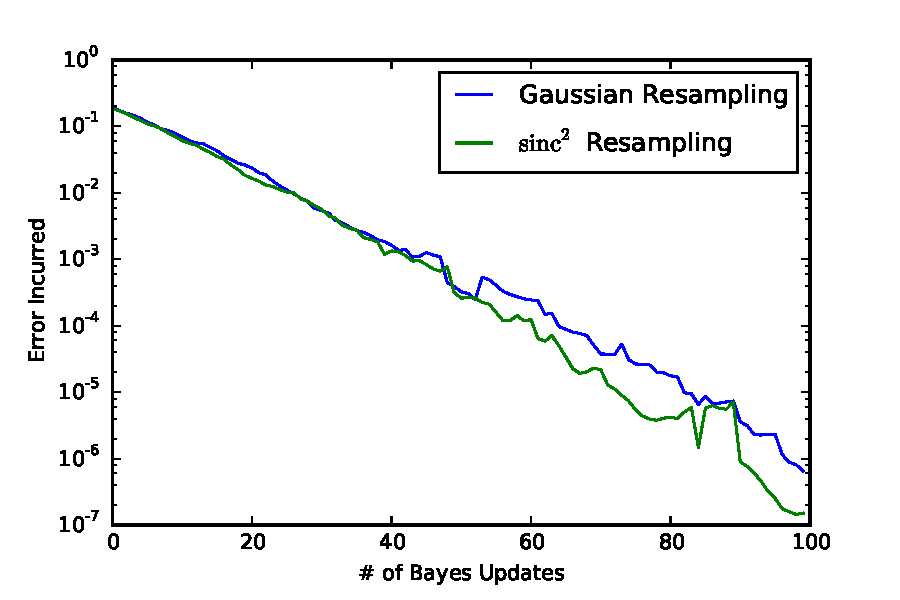
\includegraphics[width=0.6\columnwidth]{lw-sinc-resampling.pdf}
    \end{centering}
    \caption{
        \label{fig:lw-sinc-resampling}
        Performance of classical SMC with Gaussian and $\sinc^2$ resampling kernels
        for the  periodic likelihood \eq{simple-precession} and averaged over
        1,000 trials.
    }
\end{figure}

Although we do not expect the nodes of the $\sinc^2$ function to substantially impede inference, the impact of these nodes can be reduced by using a linear combination of such states.  In particular,  we can prepare linear combinations of step functions as our initial states and Fourier transform the result.
Linear combinations of states can be prepared using the circuit
    \[
      \Qcircuit @R 1em @C 1.5em {
                        \lstick{\ket{0}} & \gate{V}&\ctrl{1}&\ctrlo{1}&\gate{V^\dagger}&\qw\\
		   \lstick{\ket{\psi}} & \qw &\gate{U_1}&\gate{U_0}&\qw&\qw
},
    \]
where for some real valued $A\ge 0$~\cite{CW12} we have
\begin{equation}
V=\begin{pmatrix} \sqrt{\frac{A}{A+1}} & -\sqrt{\frac{1}{A+1}} \\ \sqrt{\frac{1}{A+1}}& \sqrt{\frac{A}{A+1}} \end{pmatrix}.
\end{equation}
This is relevant because if the top-most qubit is measured to be $0$ then the circuit performs
\begin{equation}
\ket{\psi} \rightarrow \frac{(AU_1 + U_0)\ket{\psi}}{|(AU_1 + U_0)\ket{\psi}|}.
\end{equation}
This allows linear combinations of initial states to be prepared from $\ket{0}$ with probability
\begin{equation}
P_{\rm succ} = \left|\frac{(A U_1 + U_0)\ket{0}}{A+1} \right|^2\label{eq:succprob}.
\end{equation}
Assuming $U_1 \ket{0} = \frac{1}{\sqrt{2^{k_1}}} \sum_{j=0}^{2^{k_1} -1} \ket{j}$ and $U_2 \ket{0} = \frac{1}{\sqrt{2^{k_2}}} \sum_{j=0}^{2^{k_2} -1} \ket{j}$ for ${k_2} \ge {k_1}$ then it is straight forward to see from~\eq{succprob} we have that a linear combination of two states can be formed with probability
\begin{equation}
P_{\rm succ} = \frac{\left(\frac{A}{\sqrt{2^{k_1}}} + \frac{1}{\sqrt{2^{k_2}}}\right)^2k_2 +\left(\frac{A}{\sqrt{2^{k_1}}} \right)^2(2^{k_1}-2^{k_2})}{(A+1)^2}.
\end{equation}
Since the probability of successfully combining the two unitaries via measurement and postselection is known, amplitude amplification can be used to make the process deterministic~\cite{BHT+00}.
The probability of success for the case where a polynomial number of terms are summed can also be computed and is furthermore also efficient.


%=====================================================================
\bibliographystyle{apsrev}
\bibliography{qsmc2}
%=====================================================================

\end{document}